\documentclass[12pt,a4paper]{report}
%\documentclass[10pt,a4paper,twocolumn]{report}


%%%%% preamble %%%%%

%%% use package %%%

\usepackage{amsmath,amssymb,amsfonts}
\usepackage{subfigure}
\usepackage{natbib}
\usepackage{setspace}
\usepackage{times}

%\usepackage[dvipdfm]{graphicx}
%\usepackage[dvips]{graphicx}
\usepackage[dvipdfmx]{graphicx}
%\usepackage{color}



%%% text size %%%
\setlength{\topmargin}{20mm}
\addtolength{\topmargin}{-1in}
\setlength{\textheight}{232mm}
\setlength{\headsep}{0mm}
\setlength{\headheight}{0mm}
\setlength{\topskip}{0mm}
\setlength{\oddsidemargin}{30mm}
\addtolength{\oddsidemargin}{-1in}
\setlength{\evensidemargin}{30mm}
\addtolength{\evensidemargin}{-1in}
\setlength{\textwidth}{150mm}
%\setlength{\leftmargin}{-1 in}

\renewcommand{\bibname}{References}

\doublespacing


\sloppy

%%% title information %%%L
\title{
  \Large{Master Thesis}\\[1.5cm]
  \LARGE{\bf Exploring the existence of prebiotic species:\\
    ALMA observations of amine-containing organic molecule in star-forming regions.}\\[3cm]
}
\author{
  \Large{\bf Harumi Minamoto}\\
%  \Large{}\\[0.5cm]
  \large{17M01629}\\
  \large{Nomura Laboratory}\\
  \large{Department of Earth and Planetary Sciences,\,Tokyo Institute of Technology}\\[2cm]
}
\date{\large{\bf \today}}


\newcommand\aj{The~Astronomical~Journal}%        % Astronomical Journal 
\newcommand\araa{Annual~Review~of~Astronomy~and~Astrophysics}%  % Annual Review of Astron and Astrophys 
\newcommand\apj{The~Astrophysical~Journal}%    % Astrophysical Journal ++
\newcommand\apjl{The~Astrophysical~Journal~Letters}     % Astrophysical Journal, Letters 
\newcommand\apjs{The~Astrophysical~Journal~Supplement}%    % Astrophysical Journal, Supplement 
\newcommand\ao{ApOpt}%   % Applied Optics ++
\newcommand\apss{Ap\&SS}%  % Astrophysics and Space Science 
\newcommand\aap{Astronomy~\&~Astrophysics}%     % Astronomy and Astrophysics 
\newcommand\aapr{A\&A~Rv}%  % Astronomy and Astrophysics Reviews 
\newcommand\aaps{A\&AS}%    % Astronomy and Astrophysics, Supplement 
\newcommand\azh{AZh}%       % Astronomicheskii Zhurnal 
\newcommand\baas{BAAS}%     % Bulletin of the AAS 
\newcommand\icarus{Icarus}% % Icarus
\newcommand\jrasc{JRASC}%   % Journal of the RAS of Canada 
\newcommand\memras{MmRAS}%  % Memoirs of the RAS 
\newcommand\mnras{Monthly~Notices~of~the~Royal~Astronomical~Society}%   % Monthly Notices of the RAS 
\newcommand\pra{PhRvA}% % Physical Review A: General Physics ++
\newcommand\prb{PhRvB}% % Physical Review B: Solid State ++
\newcommand\prc{PhRvC}% % Physical Review C ++
\newcommand\prd{PhRvD}% % Physical Review D ++
\newcommand\pre{PhRvE}% % Physical Review E ++
\newcommand\prl{PhRvL}% % Physical Review Letters 
\newcommand\pasp{PASP}%     % Publications of the ASP 
\newcommand\pasj{PASJ}%     % Publications of the ASJ 
\newcommand\qjras{QJRAS}%   % Quarterly Journal of the RAS 
\newcommand\skytel{S\&T}%   % Sky and Telescope 
\newcommand\solphys{SoPh}% % Solar Physics 
\newcommand\sovast{Soviet~Ast.}% % Soviet Astronomy 
\newcommand\ssr{SSRv}% % Space Science Reviews 
\newcommand\zap{ZA}%       % Zeitschrift fuer Astrophysik 
\newcommand\nat{Nature}%  % Nature 
\newcommand\iaucirc{IAUC}% % IAU Cirulars 
\newcommand\aplett{Astrophys.~Lett.}%  % Astrophysics Letters 
\newcommand\apspr{Astrophys.~Space~Phys.~Res.}% % Astrophysics Space Physics Research 
\newcommand\bain{BAN}% % Bulletin Astronomical Institute of the Netherlands 
\newcommand\fcp{FCPh}%   % Fundamental Cosmic Physics 
\newcommand\gca{Geochimica~et~Cosmochimica~Acta}% % Geochimica Cosmochimica Acta 
\newcommand\grl{Geophys.~Res.~Lett.}%  % Geophysics Research Letters 
\newcommand\jcp{JChPh}%     % Journal of Chemical Physics 
\newcommand\jgr{J.~Geophys.~Res.}%     % Journal of Geophysics Research 
\newcommand\jqsrt{JQSRT}%   % Journal of Quantitiative Spectroscopy and Radiative Trasfer 
\newcommand\memsai{MmSAI}% % Mem. Societa Astronomica Italiana 
\newcommand\nphysa{NuPhA}%     % Nuclear Physics A 
\newcommand\physrep{PhR}%       % Physics Reports 
\newcommand\physscr{PhyS}%        % Physica Scripta 
\newcommand\planss{Planetary~and~Space~Science}%  % Planetary Space Science 
\newcommand\procspie{Proc.~SPIE}%      % Proceedings of the SPIE 

\newcommand\actaa{AcA}%  % Acta Astronomica
\newcommand\caa{ChA\&A}%  % Chinese Astronomy and Astrophysics
\newcommand\cjaa{ChJA\&A}%  % Chinese Journal of Astronomy and Astrophysics
\newcommand\jcap{JCAP}%  % Journal of Cosmology and Astroparticle Physics
\newcommand\na{NewA}%  % New Astronomy
\newcommand\nar{NewAR}%  % New Astronomy Review
\newcommand\pasa{PASA}%  % Publications of the Astron. Soc. of Australia
\newcommand\rmxaa{RMxAA}%  % Revista Mexicana de Astronomia y Astrofisica

%% added feb 9, 2016
\newcommand\maps{Meteoritics~and~Planetary~Science}% Meteoritics and Planetary Science
\newcommand\aas{AAS Meeting Abstracts}% American Astronomical Society Meeting Abstracts
\newcommand\dps{AAS/DPS Meeting Abstracts}% American Astronomical Society/Division for Planetary Sciences Meeting Abstracts


%%%%% main page %%%%%
\begin{document}


%%% make title %%%
\maketitle
\thispagestyle{empty}\mbox{}\newpage

\pagenumbering{roman}

%%% abstract %%%
\chapter*{Abstract}
\addcontentsline{toc}{chapter}{Abstract}

\singlespacing



\doublespacing


%%% table of contents %%%
\tableofcontents
%\listoffigures
%\listoftables


%%% main chapters %%%
% Empty pages are inserted to make each title page
% come to the right-hand side (odd page) of the book.
\thispagestyle{empty}\mbox{}\newpage
\chapter{Introduction
  \label{chap:introduction}}

%%% page numbering %%%
\pagenumbering{arabic}

\section{Origin of life}
The interstellar medium (ISM), where more than 190 molecules ranging from simple
linear molecules to complex organic molecules (hereafter COMs) were detected, show
chemically rich environment. Astronomers usually regard the species with more than six
atoms as COMs. Not only O-bearing species, CH3OH, CH3OCH3, HCOOCH3, but also
N-bearing species such as CH3CH2CN and CH2CHCN are known COMs. In 2016, a chiral
molecule propylene oxide (CH3CHHCH2O) was detected towards Sgr B2 (N) molecular
cloud in absorption (McGuire et al. 2016). This detection implies that molecules can get
sufficient complexity, and it will accelerate surveys of other chiral molecules, like amino
acids.
From this point of view, many observations were conducted to search for prebiotic
molecules in the ISM, which might turn into the Seeds of Life when delivered to a
planetary surface. Especially, a great attention was paid to amino acids, essential building
blocks of terrestrial life; many surveys were made unsuccessfully to search for the simplest
amino acid, glycine (NH2CH2COOH), towards Sgr B2 and other high-mass star forming
regions (e.g., Brown et al. 1979; Snyder et al. 1983; Combes et al. 1996). In 2003, Kuan
et al. (2003) claimed the rst detection of glycine, however, several follow-up observations
concluded denied the detection (e.g., Jones et al. 2007). The difficulty of the past glycine
surveys would be originated from potential weakness of glycine lines and low sensitivities of
telescopes used for the surveys.

\section{Glycine and methylamine}


\section{Star forming region}
\subsection{Orion Kleinmann-Low nebula}
\subsection{IRAS 16293-2422}
\subsection{L483}

\section{Radio observation}
\subsection{Atacama Large Millimeter Array}
\subsection{Principle of interferometry}

\section{Purpose of this work}
%\thispagestyle{empty}\mbox{}\newpage
\chapter{Analysis
\label{chap:}}
%\thispagestyle{empty}\mbox{}\newpage
\chapter{Results
  \label{chap:result}}

%\subsection{Transitions}
The data obtained for CH$_{3}$NH$_{2}$ are summarized in Table \ref{tab:MAOri}.
Here the rest frequencies, product of the line strength and the dipole moment ($S\mu^2$), the upper state energy ($E_{\mathrm{u}}$), the quantum numbers, and noise level are listed.

Out of 24 selected transitions in our observational frequency range, 
6 were probably identified and are reported in Table \ref{tab:MAOri}. 
The remaining 18 CH$_{3}$NH$_{2}$ transitions are blended with or masked by other spectral features, 
or its signal are below the noise level (See Appendix~B). 

\renewcommand{\arraystretch}{1.5}
\begin{table}[htb]
\begin{center}

  \caption{Observed rotational transitions of CH$_3$NH$_2$ in Orion-KL}
  \label{tab:MAOri}
{\scriptsize
  \begin{tabular}{ccccccl} \hline
   Frequency [GHz]& S$\mu ^{2}$ [D$^2$] & E$_{\rm{u}}$ [K]& Transition ($J$, $K_{\rm{a}}$, $\Gamma$) & Noise [K] & Conversion (K to Jy/beam) &Comments \\ \hline 
    217.758 & 129.88 & 182.05 & 12, 2, $B_{2}$ $\rightarrow$ 12, 1, $B_{1}$ &  0.034 &0.847 &Reported in Pagani+17 \\
    245.202 & 37.84 & 168.31 & 12, 1, $B_{2}$ $\rightarrow$ 11, 2, $B_{1}$ & 0.037&0.069 &Reported in Pagani+17 \\
    235.735 & 82.06 & 92.76 & 8, 2, $B_{2}$ $\rightarrow$ 8, 1, $B_{1}$ &  0.081&0.073 &Reported in Pagani+17 \\
    229.908 & 27.37 & 92.71 & 8, 2, $A_{2}$ $\rightarrow$ 8, 1, $A_{1}$ & 0.064&0.051&\\ 
    242.262 & 60.23 & 60.86 & 6, 2, $B_{2}$ $\rightarrow$ 6, 1, $B_{1}$ &  0.166 &0.073&SV data \\
    244.887 & 49.54 & 48.09 & 5, 2, $B_{1}$ $\rightarrow$ 5, 1, $B_{2}$ & 0.043 &0.069&Reported in Pagani+17 \\ \hline
  \end{tabular}
  }
\end{center}
\end{table}

\newpage
\section{Overall CH$_3$NH$_2$ distribution}
Figure \ref{fig:mom0s} shows the integrated intensity maps of the 6 transitions in Table \ref{tab:MAOri} (see the procedure no.2 in section 2.2.2), and CH3NH2 emission appearsCH$_3$NH$_2$ emission appears mainly at Hot core and partially at IRc7.
According to previous work \citep[see e.g.,][]{Feng+2015, Gong+2015}, N-bearing species tend to have 
similar peak at or near Hot core.  CH$_3$NH$_2$ also shows the same trend.

Figure \ref{ch_0}-\ref{ch_5} show channel maps of expected unblended lines at 217.758~GHz, 
245.202~GHz, 229.908~GHz, 235.735~GHz, 242.262~GHz, 244.887~GHz, respectively.
The channel maps enable us to confirm the region where the radiations of molecules come and its velocity component.

In the integrated intensity map of 229.908 GHz line, emission come from the southern part of Hot core (Figure \ref{fig:mom0s}).
Since it can be confirmed that the velocity component is different in the channel map (see Figure \ref{ch_3}), 
this is considered to be the emission of another molecular line.

In addition, the extended emission in Hot core and the compact structure at Compact ridge are seen 
in the integrated intensity map of 242.262 GHz line (Figure \ref{fig:mom0s}). 
These are also considered to be emission from other molecule line 
by the channel map (Figure \ref{ch_5}) and spectrum (Figure 3.8).

\newpage
%%%%% 積分強度図挿入 %%%%%
\begin{figure}[H] 
\begin{center}
\begin{minipage}{0.98\textwidth} 
\begin{center}
%%%% ここから
\begin{minipage}{0.48\textwidth}
\begin{center}
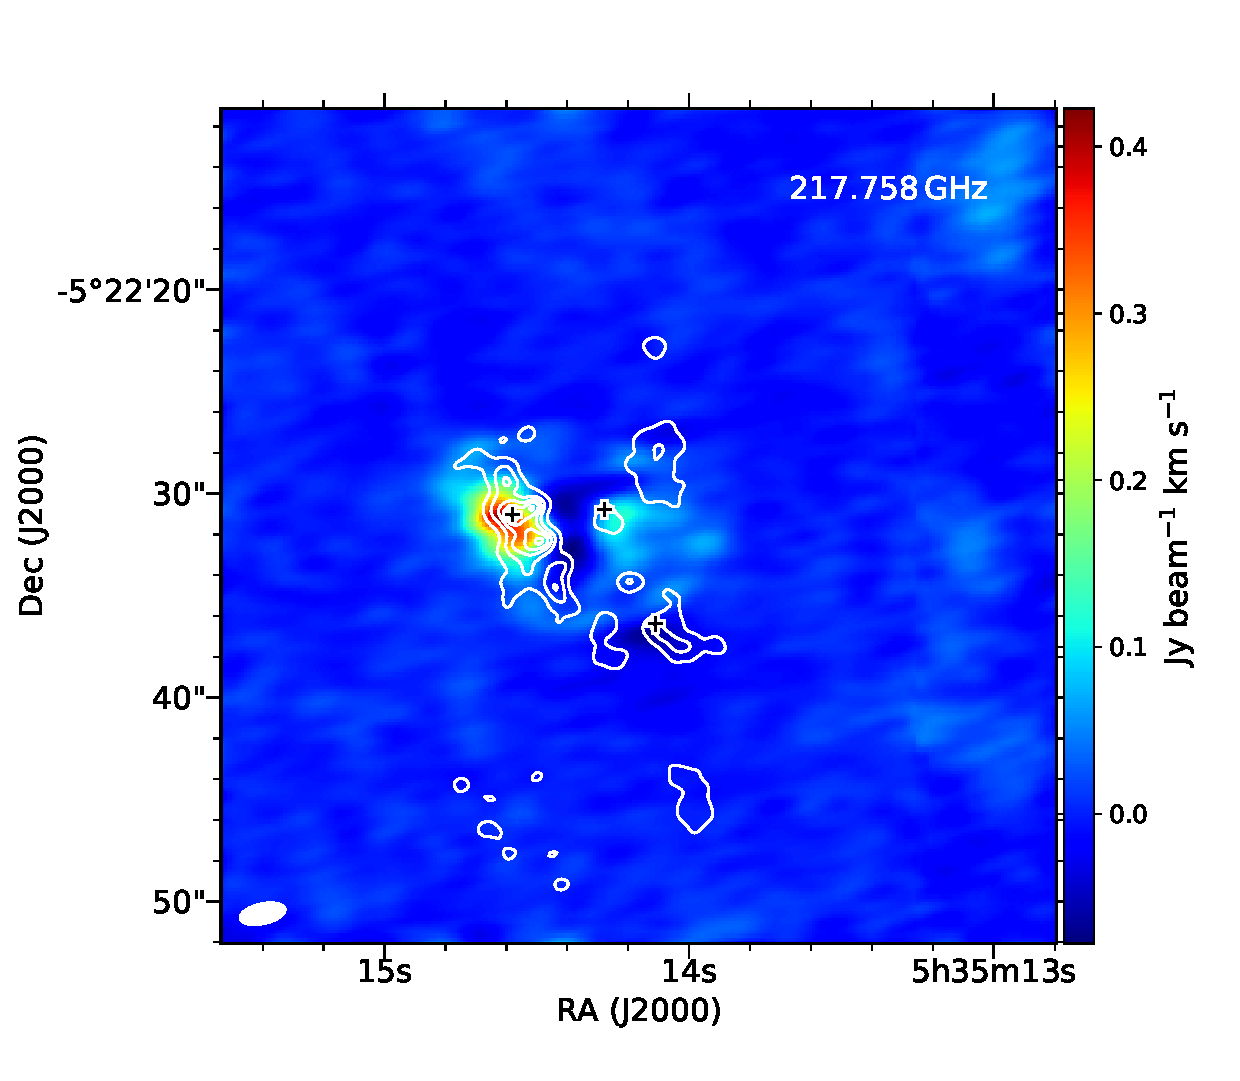
\includegraphics[width=0.98\textwidth]{OrionKL/mom0/217.758mom0_3-7.eps}
%\\(a) 左の図の説明
\end{center}
\end{minipage}
\begin{minipage}{0.48\textwidth}
\begin{center}
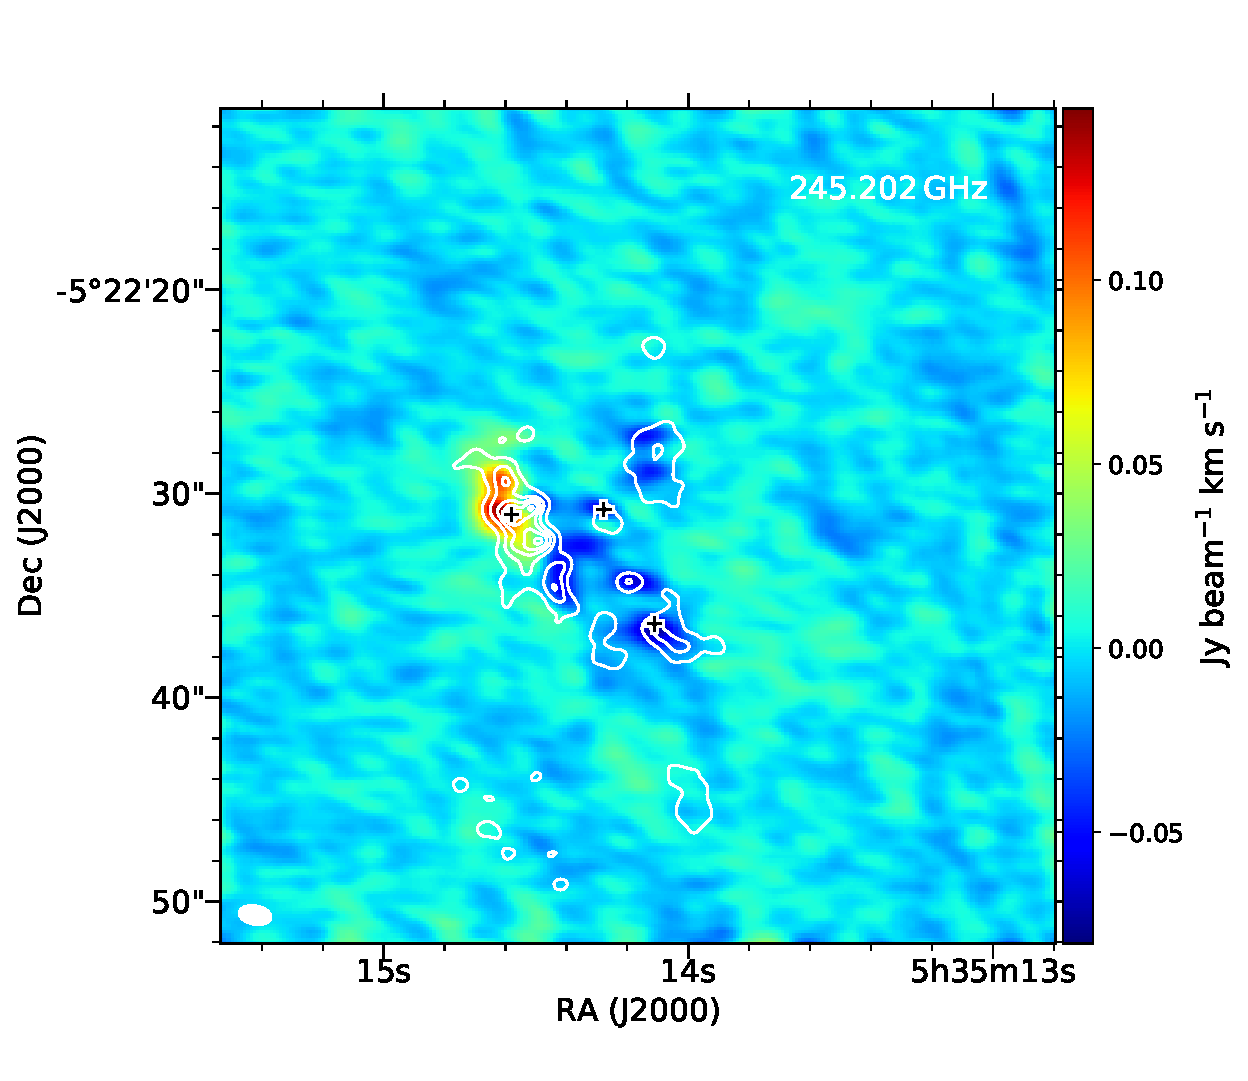
\includegraphics[width=0.98\textwidth]{OrionKL/mom0/245.202mom0_3-7.eps}
%\\(b) 右の図の説明
\end{center}
\end{minipage}
\end{center}
\end{minipage}
%%%% ここまで一組

%\begin{minipage}{0.98\textwidth} 
%\begin{center}
%\begin{minipage}{0.48\textwidth}
%\begin{center}
%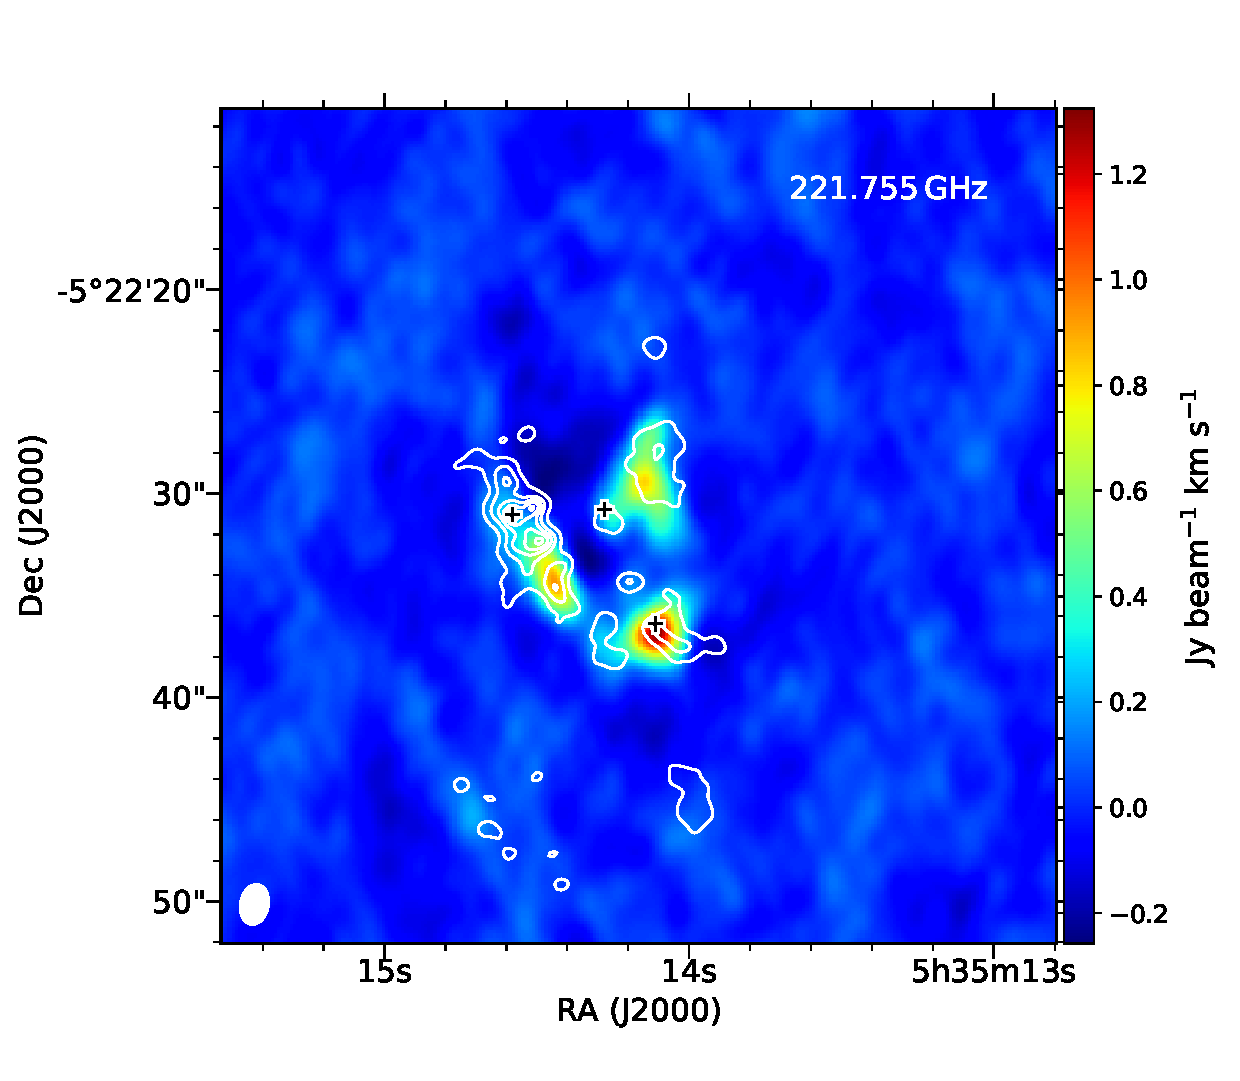
\includegraphics[width=0.98\textwidth]{OrionKL/mom0/221.755SV_mom0_3-7.eps}
%\\(c) 左の図の説明
%\end{center}
%\end{minipage}
%\begin{minipage}{0.48\textwidth}
%\begin{center}
%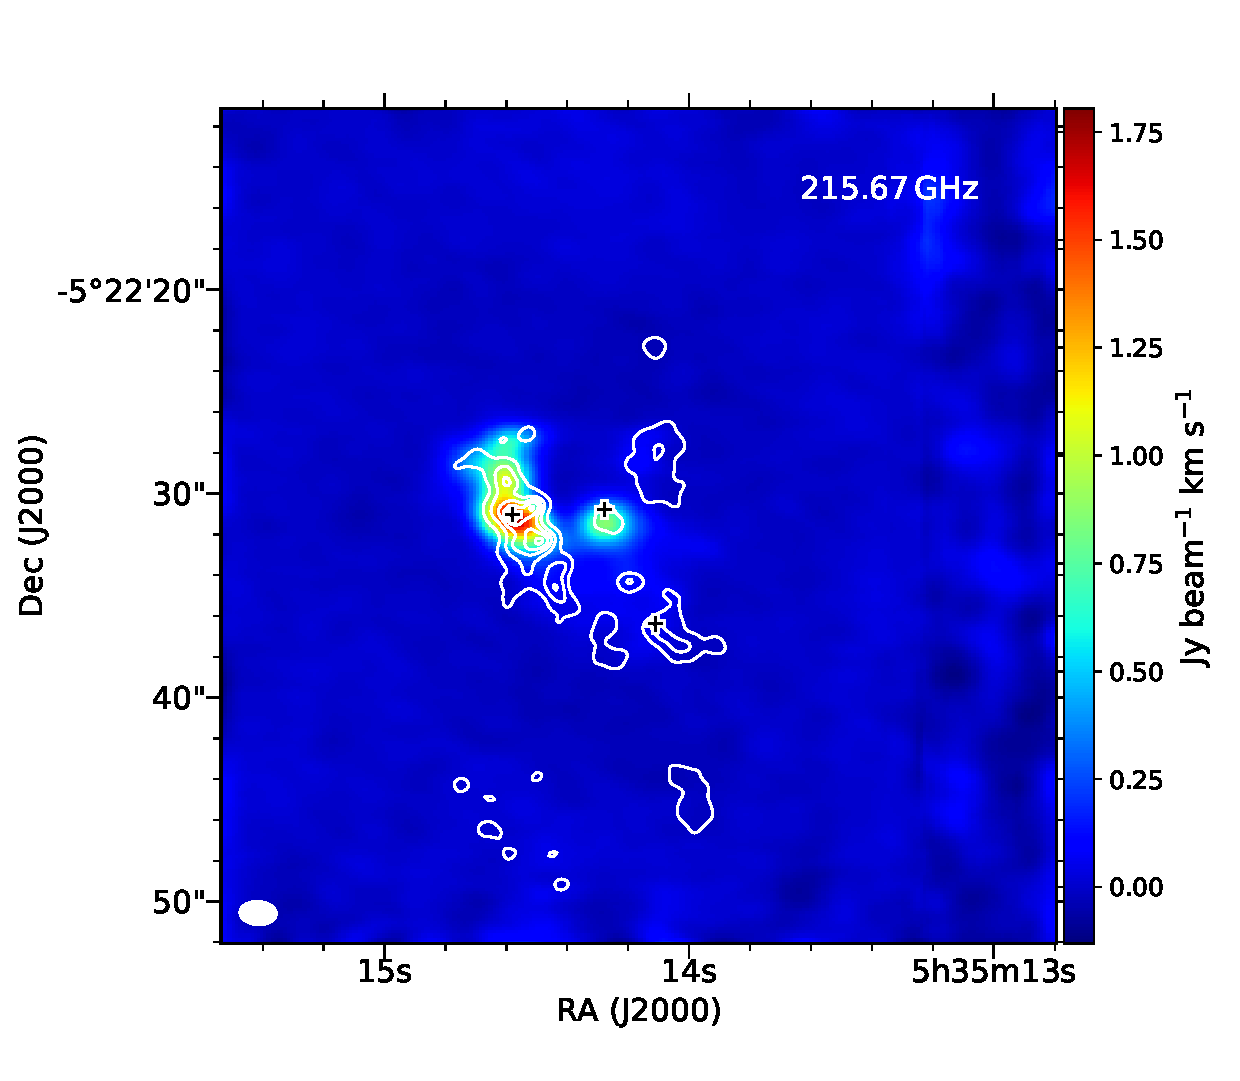
\includegraphics[width=0.98\textwidth]{OrionKL/mom0/215.67mom0_3-7.eps}
%\\(d) 右の図の説明
%\end{center}
%\end{minipage}
%\end{center}
%\end{minipage}
%\end{center}
%\end{figure}

%\begin{figure}[H] 
%\begin{center}
\begin{minipage}{0.98\textwidth} 
\begin{center}
%%%% ここから
\begin{minipage}{0.48\textwidth}
\begin{center}
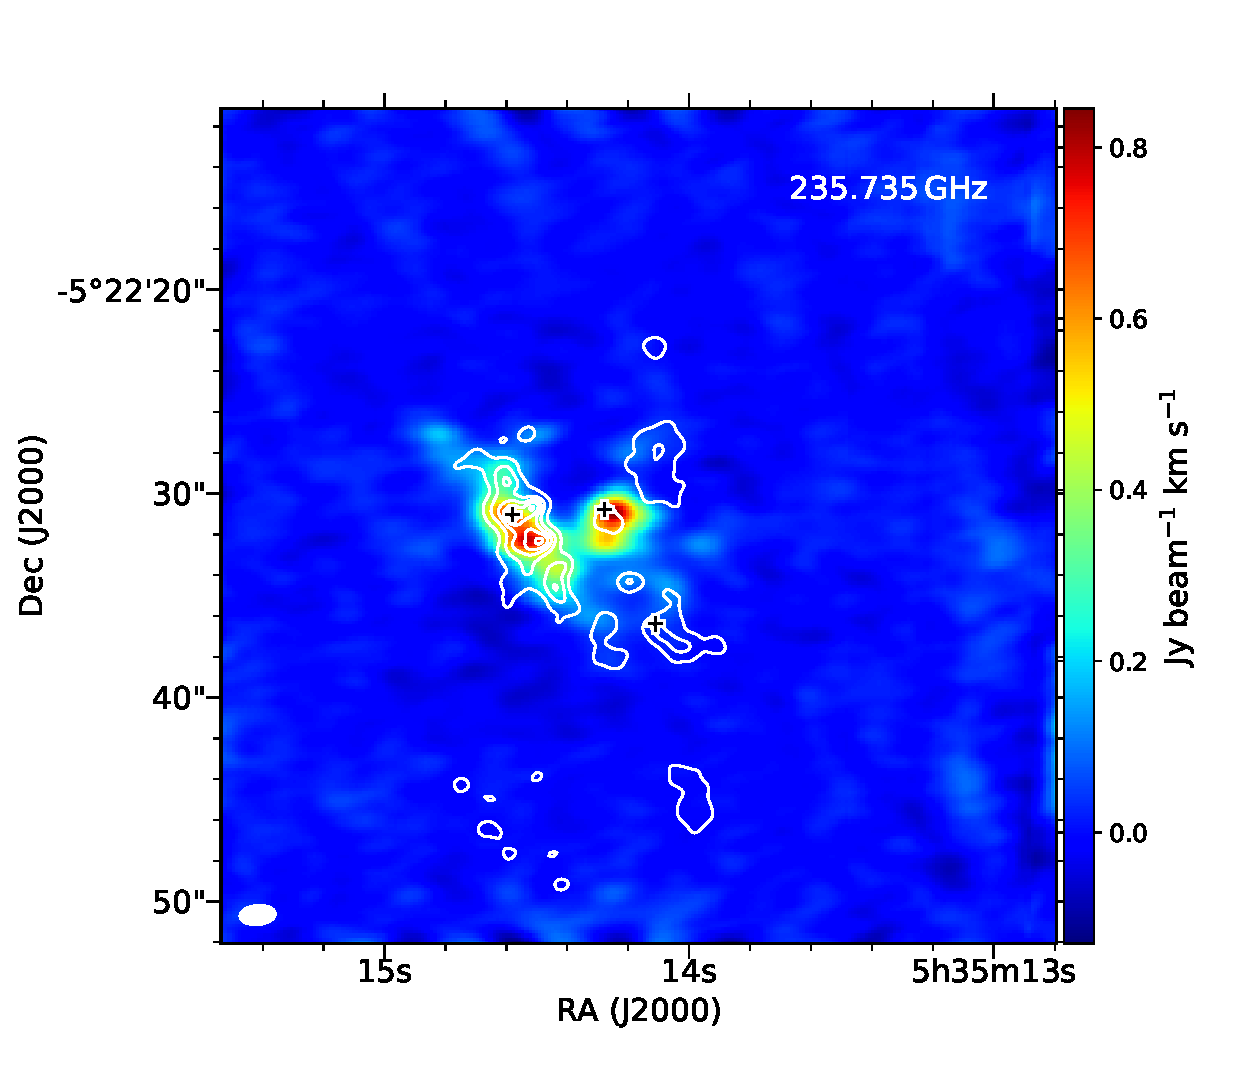
\includegraphics[width=0.98\textwidth]{OrionKL/mom0/235.735mom0_3-7.eps}
%\\(e) 左の図の説明
\end{center}
\end{minipage}
\begin{minipage}{0.48\textwidth}
\begin{center}
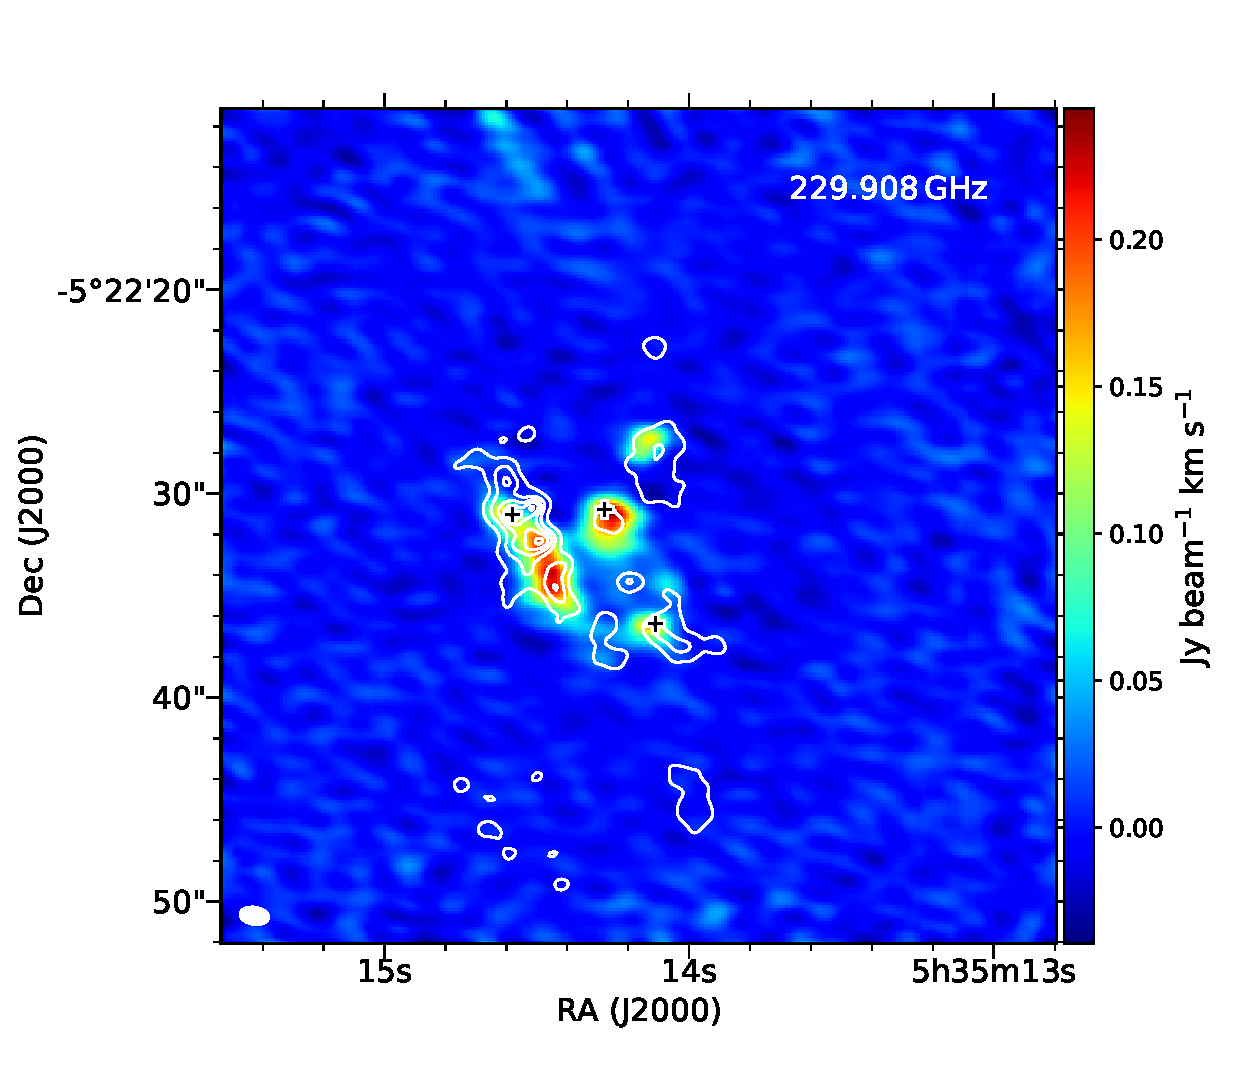
\includegraphics[width=0.98\textwidth]{OrionKL/mom0/229.908mom0_3-7.eps}
%\\(f) 右の図の説明
\end{center}
\end{minipage}
\end{center}
\end{minipage}
%%%% ここまで一組

\begin{minipage}{0.98\textwidth} 
\begin{center}
\begin{minipage}{0.48\textwidth}
\begin{center}
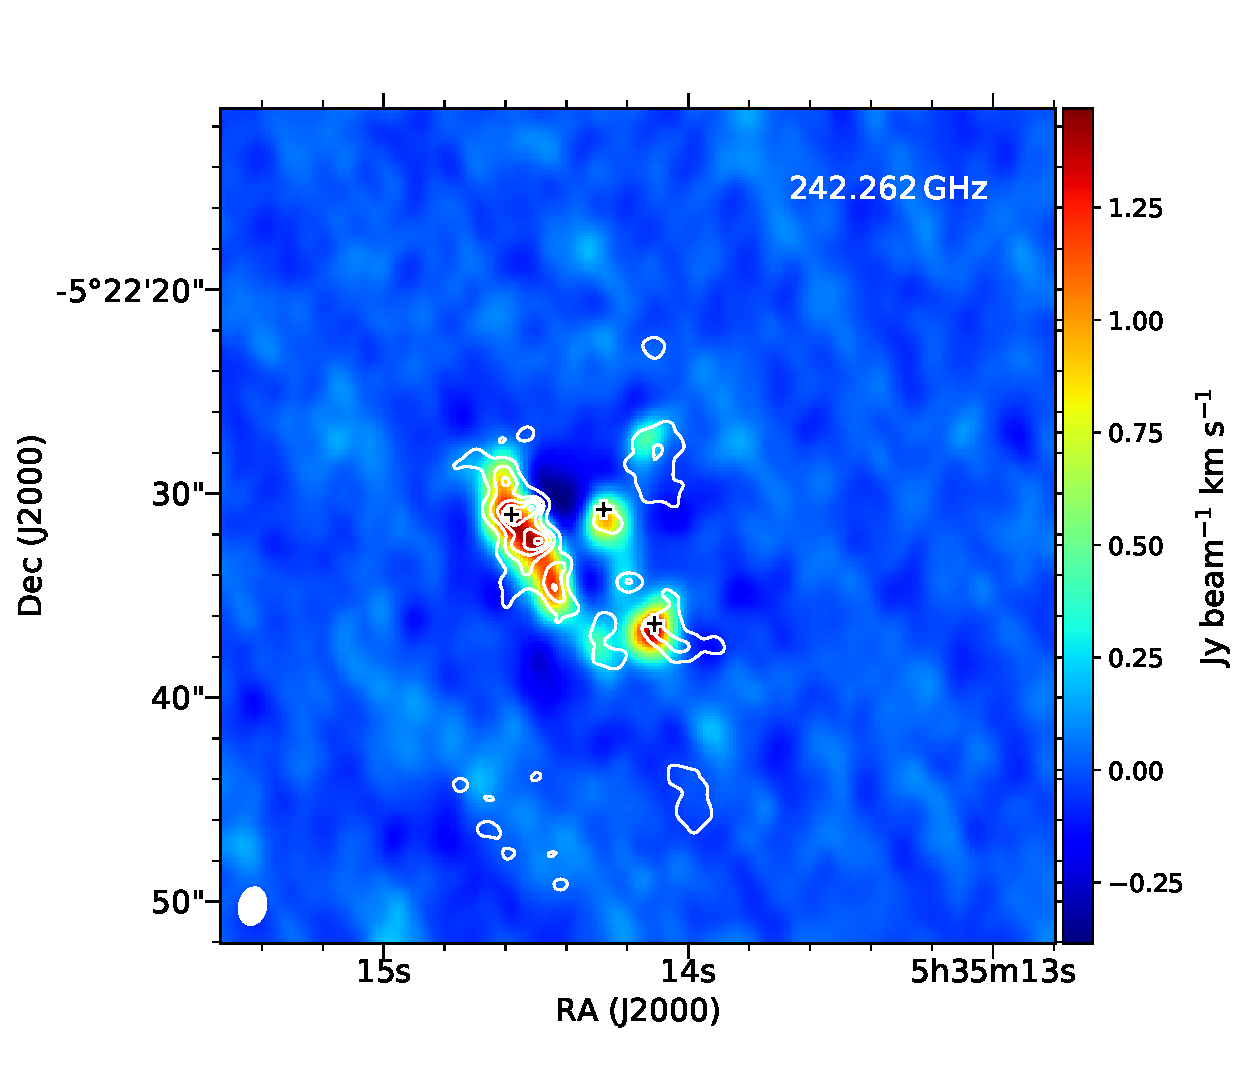
\includegraphics[width=0.98\textwidth]{OrionKL/mom0/242.262SV_mom0_3-7.eps}
%\\(g) 左の図の説明
\end{center}
\end{minipage}
\begin{minipage}{0.48\textwidth}
\begin{center}
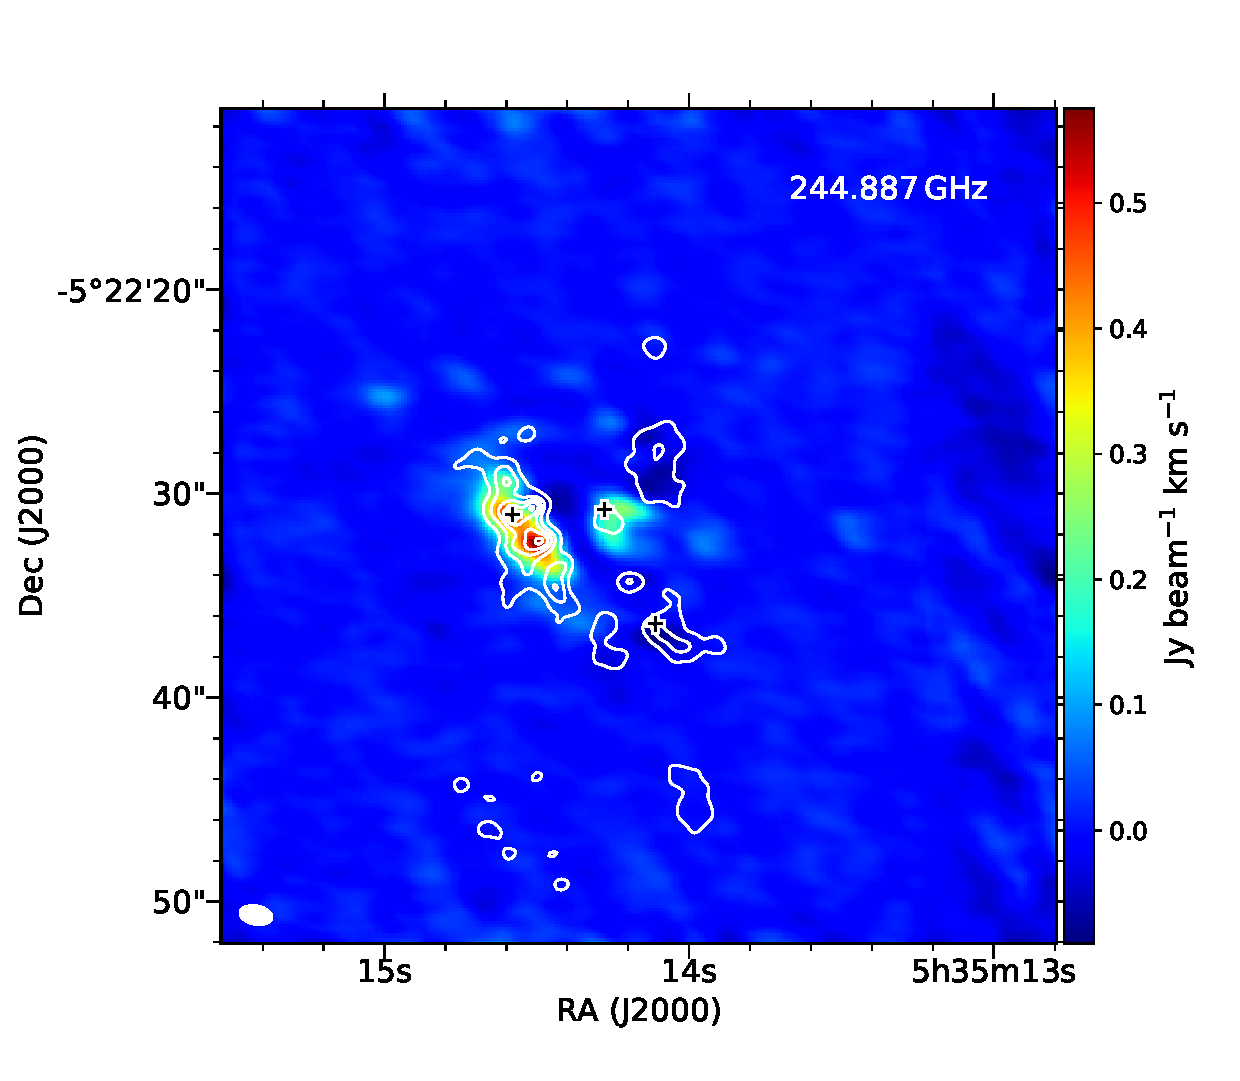
\includegraphics[width=0.98\textwidth]{OrionKL/mom0/244.887mom0_3-7.eps}
%\\(h) 右の図の説明
\end{center}
\end{minipage}
\end{center}
\end{minipage}

\label{fig:mom0s}
\caption{Integrated intensity maps of unblended CH$_{3}$NH$_{2}$ lines. 
The white contours show the 1.3 mm continuum map from \citet{Hirota+2015},
where the contour levels are 10 \%, 30 \%, 50 \%, 70 \%, 90 \% of the peak intensity of 0.40 Jy/beam.
Same as Figure \ref{fig:cont+2015} but for black crosses. The rest frequency of each transition shows in the upper right part of each panel.}
%\caption{(Continued)}
\end{center}
\end{figure}
%%%%% 積分強度図ここまで %%%%%

%%%%%% チャネルマップここから
\begin{figure}[H]
  \centering
  \includegraphics[width=0.98\textwidth]{OrionKL/chmap/217.758.eps}
  \caption{
  Channel map of expected unblended 217.758 GHz line show multiple velocity-dependent 
  emission peaks: 4-6 km s$^{-1}$ towards Hot core, 7-9km s$^{-1}$ towards IRc7. 
  Magenta crosses denote Hot core, IRc7, and Compact ridge. Same as Figure \ref{fig:cont+2015} but for white contours.}
  \label{ch_0}
\end{figure}

\begin{figure}[H]
  \centering
  \includegraphics[width=0.98\textwidth]{OrionKL/chmap/245.202.eps}
  \caption{Channel map of expected unblended 245.202 GHz line.}
  \label{ch_1}
\end{figure}

\begin{figure}[H]
  \centering
  \includegraphics[width=0.98\textwidth]{OrionKL/chmap/235.735.eps}
  \caption{Channel map of expected unblended 235.735 GHz line.}
  \label{ch_2}
\end{figure}

\begin{figure}[H]
  \centering
  \includegraphics[width=0.98\textwidth]{OrionKL/chmap/229.908.eps}
  \caption{Channel map of expected unblended 229.908 GHz line.}
  \label{ch_3}
\end{figure}

\begin{figure}[H]
  \centering
  \includegraphics[width=0.98\textwidth]{OrionKL/chmap/242.262.eps}
  \caption{Channel map of expected unblended 242.262 GHz line.}
  \label{ch_4}
\end{figure}

\begin{figure}[H]
  \centering
  \includegraphics[width=0.98\textwidth]{OrionKL/chmap/244.887.eps}
  \caption{Channel map of expected unblended 244.887 GHz line.}
  \label{ch_5}
\end{figure}

\newpage
\section{Spectra}
Figure 3.8 shows the spectra of the CH$_3$NH$_2$ lines extracted from Hot core.
The spectrum were extracted from the region of $1''.0$ in diameter around 
Hot core (RA$_{J2000}: 05^{\rm{h}}35^{\rm{m}}14^{\rm{s}}.580$, Dec$_{J2000}:-05^{\circ}22'31''.029$), 
and the Gaussian fitting was performed to obtain FWHM line widths and the mean local standard of 
rest velocity $V_{\mathrm{LSR}}$ of the emission lines.
The line measurements toward Hot core are listed in Table \ref{tab:paraOri}.


The average LSR velocity and FWHM line width are estimated to be 4.84~$\pm$~0.22~km~s$^{-1}$ and 
4.16~$\pm$~0.79~km~s$^{-1}$, respectively.
 $V_{\mathrm{LSR}}$ are consistent with those reported by \citet{Feng+2015} 
 for N-bearing COMs observed toward Hot core
 (e.g, 4.9~km~s$^{-1}$ for CH$_2$CHCN, 5.1~km~s$^{-1}$ for CH$_3$CH$_2$CN).
On the other hand, $\Delta V_{1/2}$ of CH$_3$NH$_2$ is narrower than those of other molecule in Hot core
\citep[typically 5--15~km~s$^{-1}$,][]{Pagani+2017}.

\renewcommand{\arraystretch}{1.5}
\begin{table}[htb]
\begin{center}

  \caption{CH$_3$NH$_2$ line parameters toward Hot core}
  \label{tab:paraOri}
{\scriptsize
  \begin{tabular}{ccccccl} \hline
   Frequency [GHz]& E$_{\rm{u}}$ [K] &  peak $T_{\mathrm{B}}$\footnotemark[1] [K] & $V_{\mathrm{LSR}}$\footnotemark[1] [km s$^{-1}$] & $\Delta V_{1/2}$\footnotemark[1] [km s$^{-1}$] & Noise [K]  & Note \\ \hline 
    217.758  & 182.05 &  0.86(0.03) & 4.73(0.08) & 3.99(0.24) & 0.034 & \\
    245.202 & 168.31 & 0.37(0.01) & 4.51(0.08) & 3.86(0.33) & 0.037 & \\
    229.908  & 92.71 &  0.65(0.01) & 4.91(0.03) & 3.19(0.06)& 0.064&\\ 
    235.735  & 92.76 & 1.70(0.02) & 4.86(0.03) & 5.60(0.10)& 0.081 & \\
    242.262  & 60.86 &  2.03(0.03) & 4.80(0.09) & 8.04(0.23) & 0.166 & Partially blended \\
    244.887  & 48.09 & 1.29(0.57)& 5.23(0.90) & 4.16(2.12) & 0.043 & \\ \hline
  \end{tabular}
  }
\end{center}
\end{table}
\footnotetext[1]{Numbers in parenthesis represent standard deviation in the unit of the last significant digits.}

Please note that the spectrum in Figure \ref{fig:spec} is superimposed with the result of the Gaussian fitting 
assuming the average $\Delta V_{1/2} = 4.2\, \mathrm{km\,s^{-1}}$.

%%%%% スペクトル挿入 %%%%%
\begin{figure}[H] 
\begin{center}
\begin{minipage}{0.98\textwidth} 
\begin{center}
%%%% ここから
\begin{minipage}{0.48\textwidth}
\begin{center}
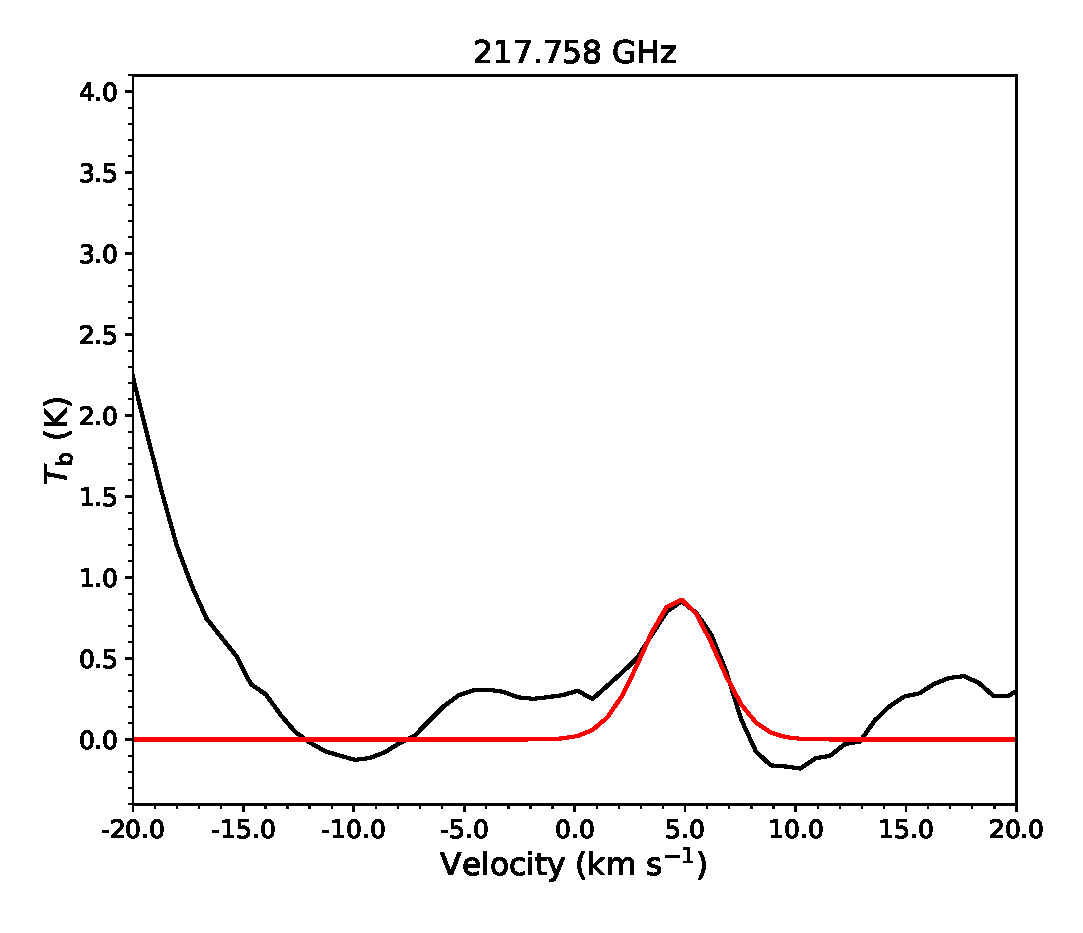
\includegraphics[width=0.98\textwidth]{OrionKL/spectrum/HC/217.758328w_fit.eps}
%\\(a) 左の図の説明
\end{center}
\end{minipage}
\begin{minipage}{0.48\textwidth}
\begin{center}
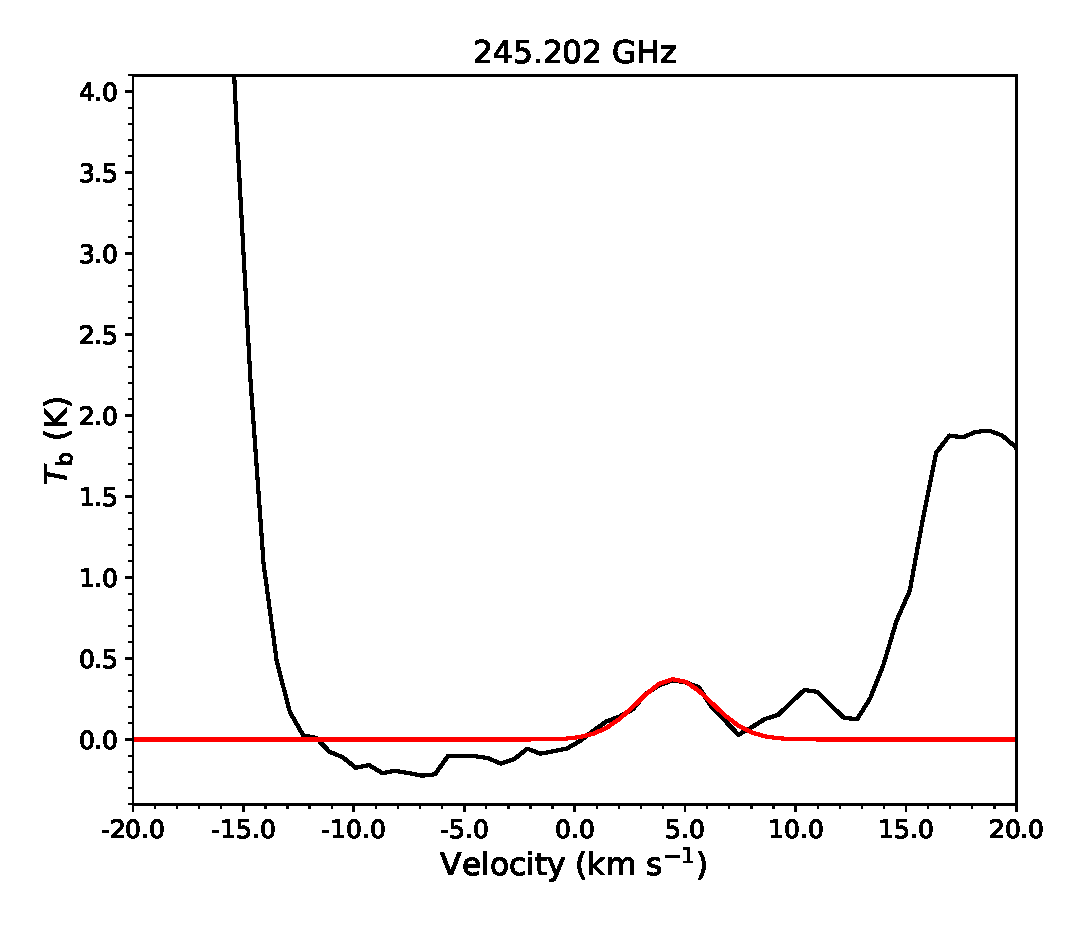
\includegraphics[width=0.98\textwidth]{OrionKL/spectrum/HC/245.2021362w_fit.eps}
%\\(b) 
\end{center}
\end{minipage}
\end{center}
\end{minipage}
%%%% ここまで一組

%\begin{minipage}{0.98\textwidth} 
%\begin{center}
%\begin{minipage}{0.48\textwidth}
%\begin{center}
%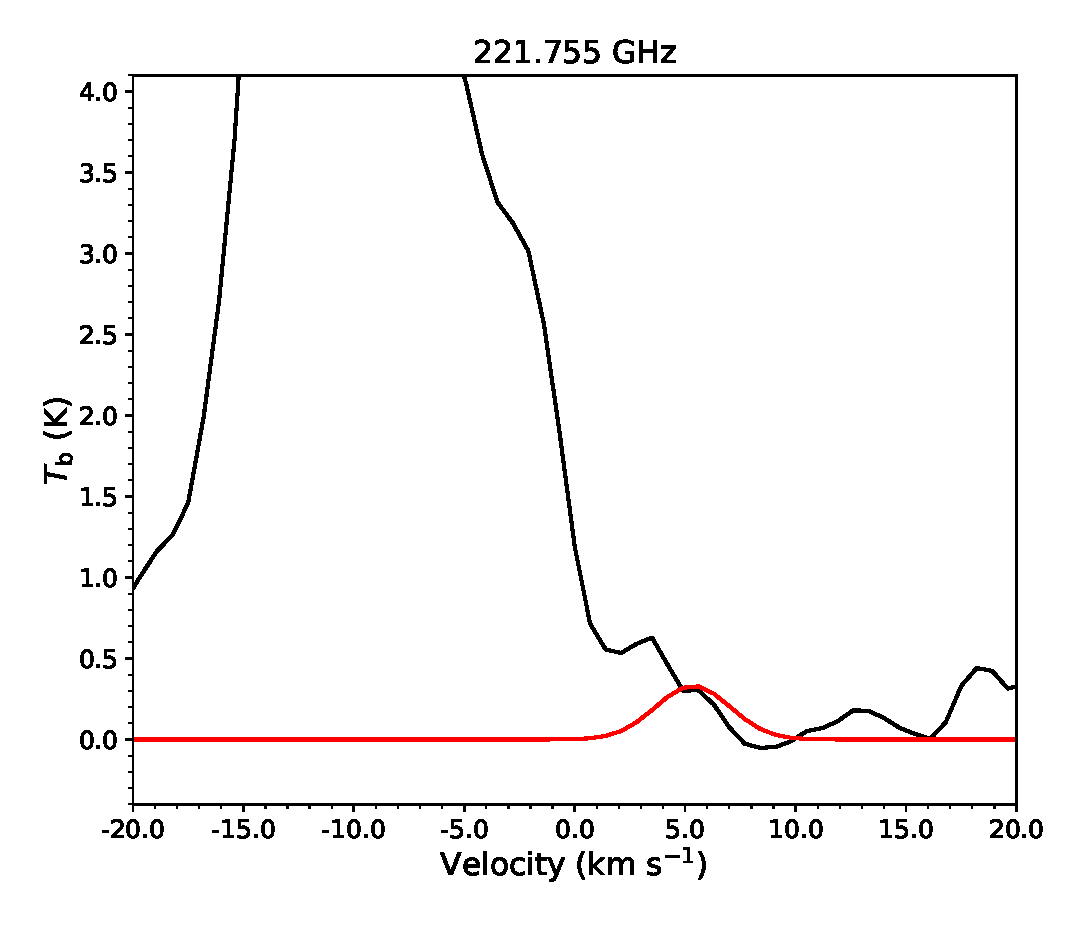
\includegraphics[width=0.98\textwidth]{OrionKL/spectrum/HC/221.755055w_fit.eps}
%\\(c) 左の図の説明
%\end{center}
%\end{minipage}
%\begin{minipage}{0.48\textwidth}
%\begin{center}
%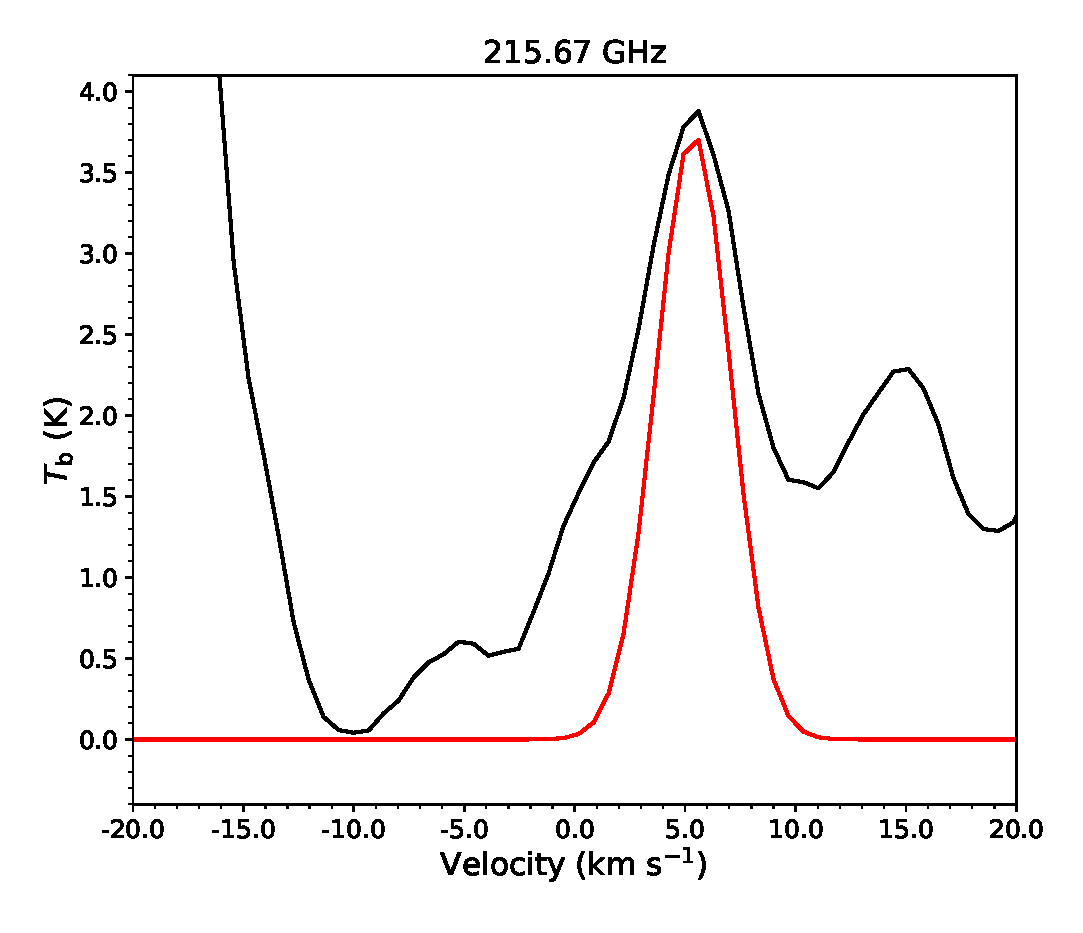
\includegraphics[width=0.98\textwidth]{OrionKL/spectrum/HC/215.6696452w_fit.eps}
%\\(d) 右の図の説明
%\end{center}
%\end{minipage}
%\end{center}
%\end{minipage}
\begin{minipage}{0.98\textwidth} 
\begin{center}
%%%% ここから
\begin{minipage}{0.48\textwidth}
\begin{center}
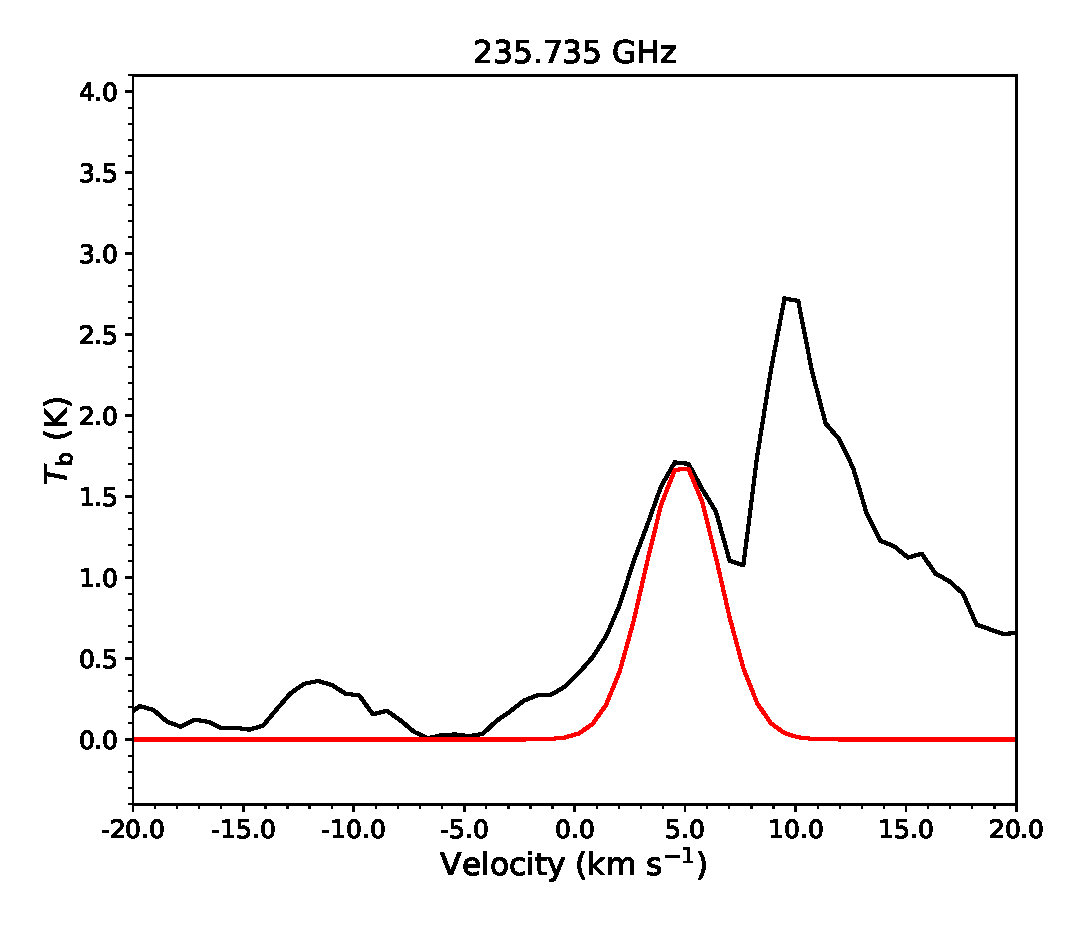
\includegraphics[width=0.98\textwidth]{OrionKL/spectrum/HC/235.735037w_fit.eps}
%\\(e) 左の図の説明
\end{center}
\end{minipage}
\begin{minipage}{0.48\textwidth}
\begin{center}
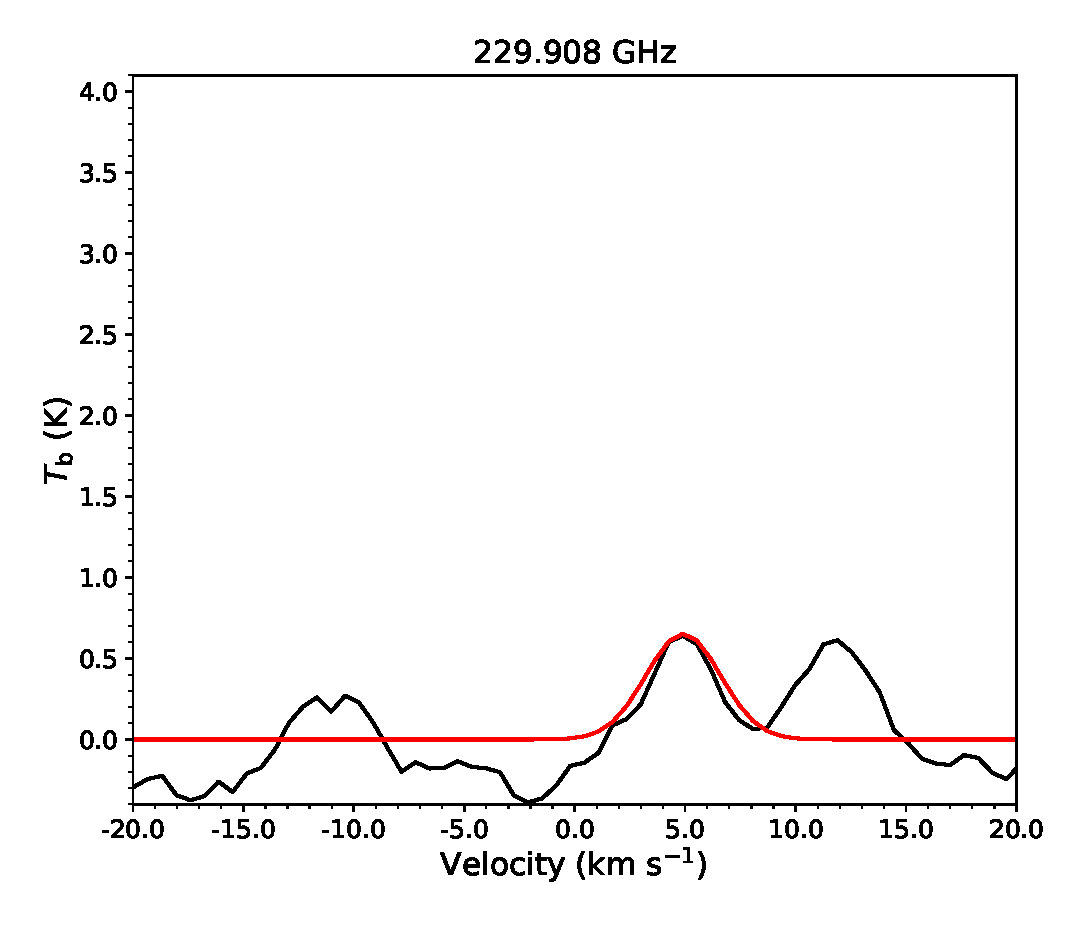
\includegraphics[width=0.98\textwidth]{OrionKL/spectrum/HC/229.908118w_fit.eps}
%\\(f) 右の図の説明
\end{center}
\end{minipage}
\end{center}
\end{minipage}
%%%% ここまで一組

\begin{minipage}{0.98\textwidth} 
\begin{center}
\begin{minipage}{0.48\textwidth}
\begin{center}
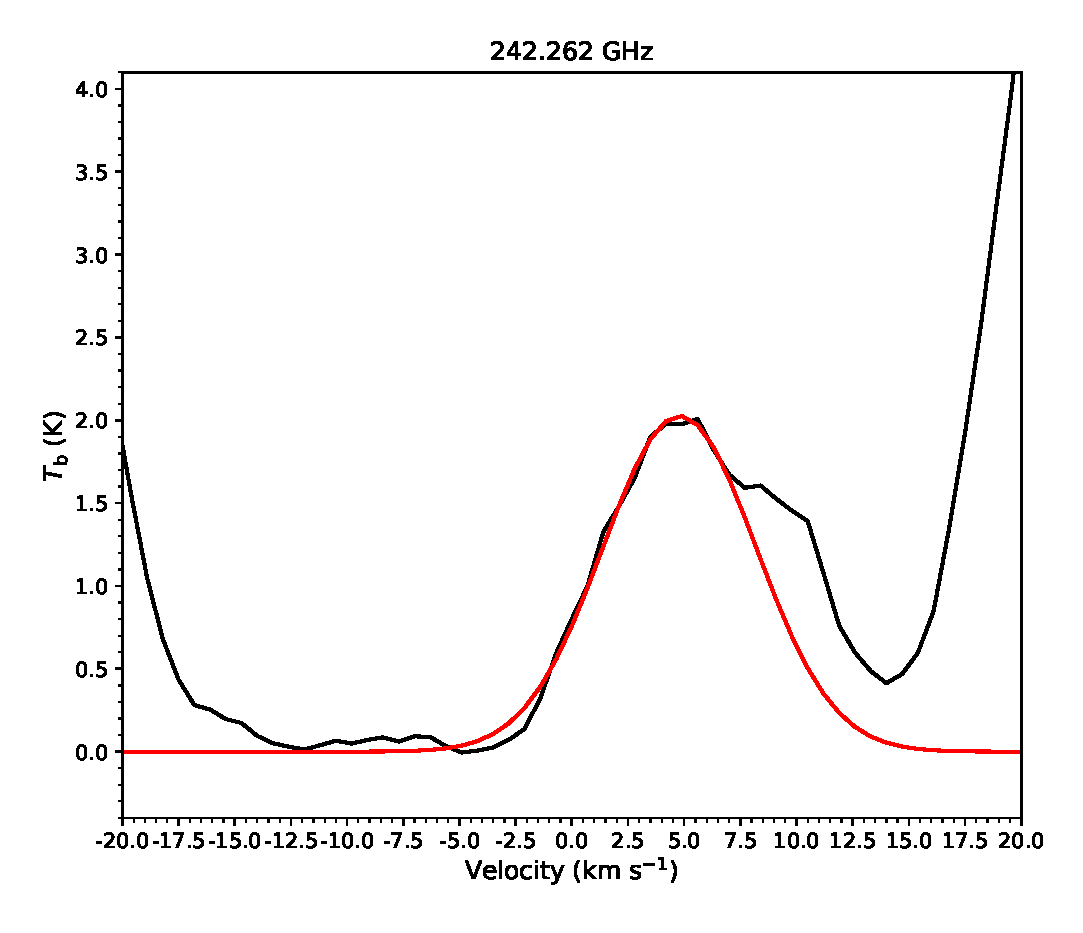
\includegraphics[width=0.98\textwidth]{OrionKL/spectrum/HC/242.2620195w_fit.eps}
%\\(g) 左の図の説明
\end{center}
\end{minipage}
\begin{minipage}{0.48\textwidth}
\begin{center}
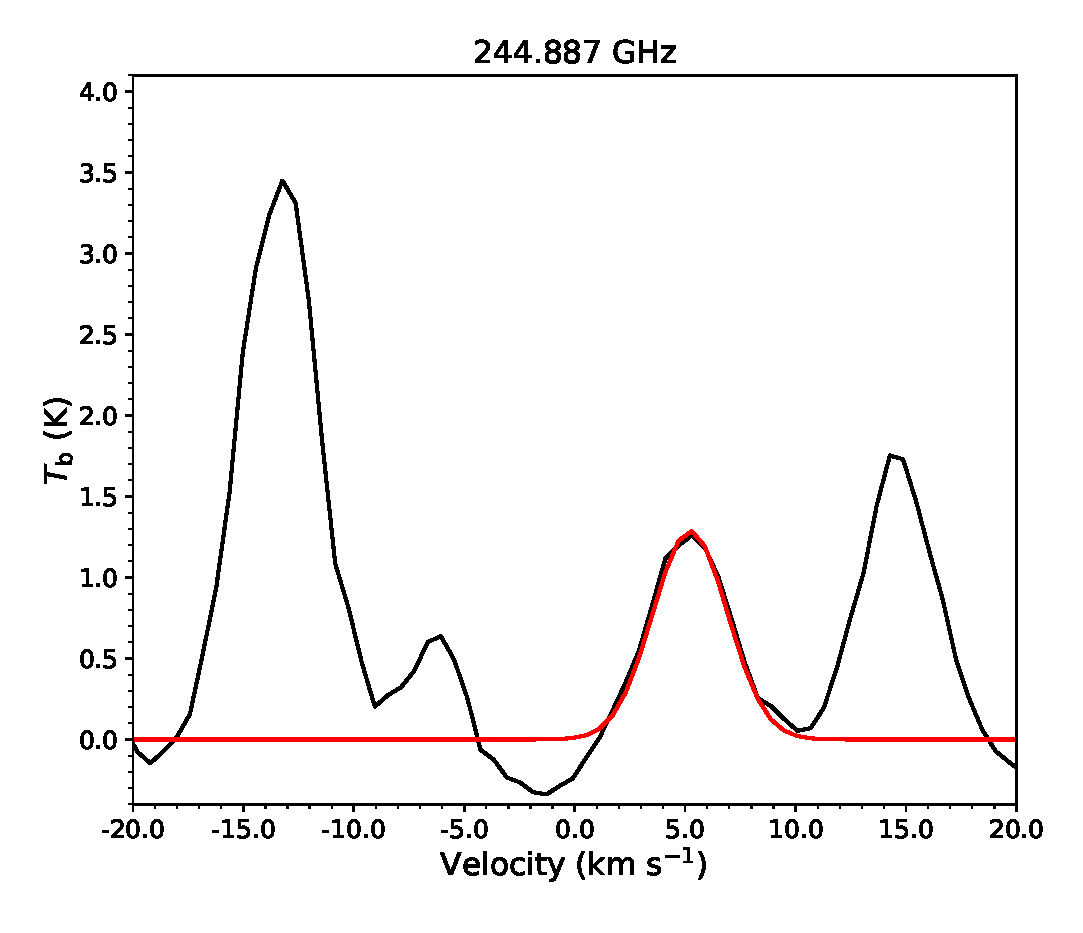
\includegraphics[width=0.98\textwidth]{OrionKL/spectrum/HC/244.8869007w_fit.eps}
%\\(h) 右の図の説明
\end{center}
\end{minipage}
\end{center}
\end{minipage}

\label{fig:spec}
\caption{Spectrum of the CH$_3$NH$_2$ lines at each frequency observed in Hot core (black) 
 and the result of the Gaussian fitting assuming the average $\Delta V_{1/2} = 4.2\, \mathrm{km\,s^{-1}}$ (red).}
\end{center}
\end{figure}

%\thispagestyle{empty}\mbox{}\newpage
\chapter{Discussion
  \label{chap:discussion}}

\section{Column density and Rotation temperature}

In this subsection we will describe the methodologies in deriving the column density and the rotational temperature of COMs.
The column density of CH$_{3}$NH$_{2}$ ($N_{\mathrm{MA}}$) was estimated by using 
the rotational temperature diagram method, which assumes local thermodynamic equilibrium 
(LTE) and optically thin emission. 
The following equation was employed for the analysis \citep{Turner1991}:
\begin{align}
\log \dfrac{3\,k_{\mathrm{B}}\,T_{\mathrm{B}} \,\Delta V_{1/2}}{8\, \pi^3\, \nu\, S\, \mu_0^2} = \log \dfrac{N_{\mathrm{MA}}}{U_{\mathrm{rot}}} - \dfrac{E_{\mathrm{u}}}{k_{\mathrm{B}}} \dfrac{\log e}{T_{\mathrm{rot}}}
\label{eq:RD}
\end{align}

In the expression, $\nu$ is the rest frequency of the transition, $\mu_0$ is the permanent dipole moment, 
$U_{\mathrm{rot}}$ is the rotational partition function, $S$ is the line strength, 
$E_{\mathrm{u}}$ is the upper state energy, and $ T_{\mathrm{B}}$ and  $\Delta V_{1/2}$ 
are the brightness temperature and line widths (FWHM, in~km~s$^{-1}$), respectively.
We assumed the average $\Delta V_{1/2} = 4.2\, \mathrm{km\,s^{-1}}$, which derived by the Gaussian fitting.

The brightness temperature can be converted from intensity $I_{\mathrm{\nu}}$
when the Rayleigh-Jeans law is applicable.
\begin{align}
T_{\mathrm{B}} = \dfrac{c^2}{2\,k_{\mathrm{B}}\, \nu^2} \,I_{\mathrm{\nu}}
\end{align}

\begin{figure}[H]
  \centering
  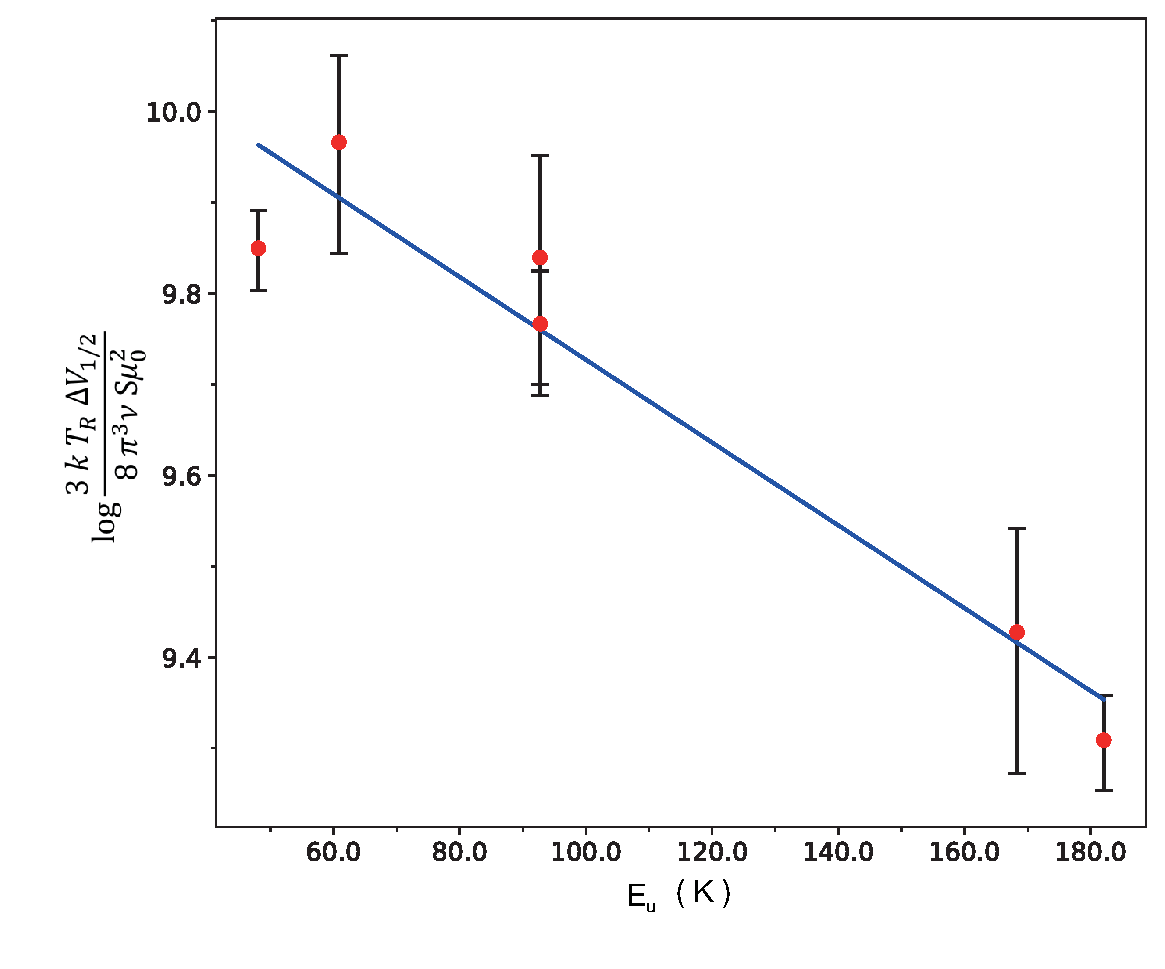
\includegraphics[width=0.8\textwidth]{OrionKL/RD_6point_label.eps}
  \caption{Rotation diagram of CH$_{3}$NH$_{2}$ in Hot core. The error bars represents $\pm$ 3 $\sigma$ for each data.}
  \label{fig:RD}
\end{figure}

The resulting plots are given in Figure \ref{fig:RD}.
The analysis yields a rotational temperature of $T_{\mathrm{rot}} =  95.4^{+15.5}_{-11.7} \,\,\mathrm{K}$, 
with a column density of $N_{\mathrm{MA}} = ( 5.5^{+1.6}_{-1.1} ) \times 10^{14} \,\,\mathrm{cm^{-2}}$.

\section{Suspicious lines}
Comparison of catalogs did not suggest contamination, but some emission lines could not be detected as CH$_{3}$NH$_{2}$.

\renewcommand{\arraystretch}{1.5}
\begin{table}[htb]
\begin{center}

  \caption{transitions of CH$_3$NH$_2$}
  \label{tab:unresolved}
{\scriptsize
  \begin{tabular}{ccccccccl} \hline
   Frequency & S$\mu ^{2}$ & E$_{\rm{u}}$& Transition & peak $T_{\mathrm{B}}$\footnotemark[1] & $V_{\mathrm{LSR}}$\footnotemark[1]  & Noise & Conversion  & Comments \\ 
  $\,$ [GHz]  & [D$^2$] &  [K] & ($J$, $K_{\rm{a}}$, $\Gamma$)  & [K] & [km s$^{-1}$] & [K] &  (K to Jy beam$^{-1}$) &  \\ \hline 
    215.670 & 53.92 & 111.48 & 9, 2, $E_{1-1}$ $\rightarrow$ 9, 1, $E_{1+1}$  & 3.74(0.07) & 5.37(0.07) & 0.043 & 0.077 &  \\
    221.755 & 35.06 & 133.11 & 10, 2, $A_{2}$ $\rightarrow$ 10, 1, $A_{1}$ & 0.33(0.03)& 5.35(0.19) & 0.133 &0.108 &SV data \\ \hline
  \end{tabular}
  }
\end{center}
\end{table}
\footnotetext[1]{Numbers in parenthesis represent standard deviation in the unit of the last significant digits.}


As shown in Figure \ref{fig:RD_blend}, the CH$_{3}$NH$_{2}$ data including 2 transitions in Table \ref{tab:unresolved} 
produced point-to-point scatter perhaps because of the lower signal-to-noise ratio for the weaker transitions in SV data 
and possible high-level contamination.

\begin{figure}[htp]
  \centering
  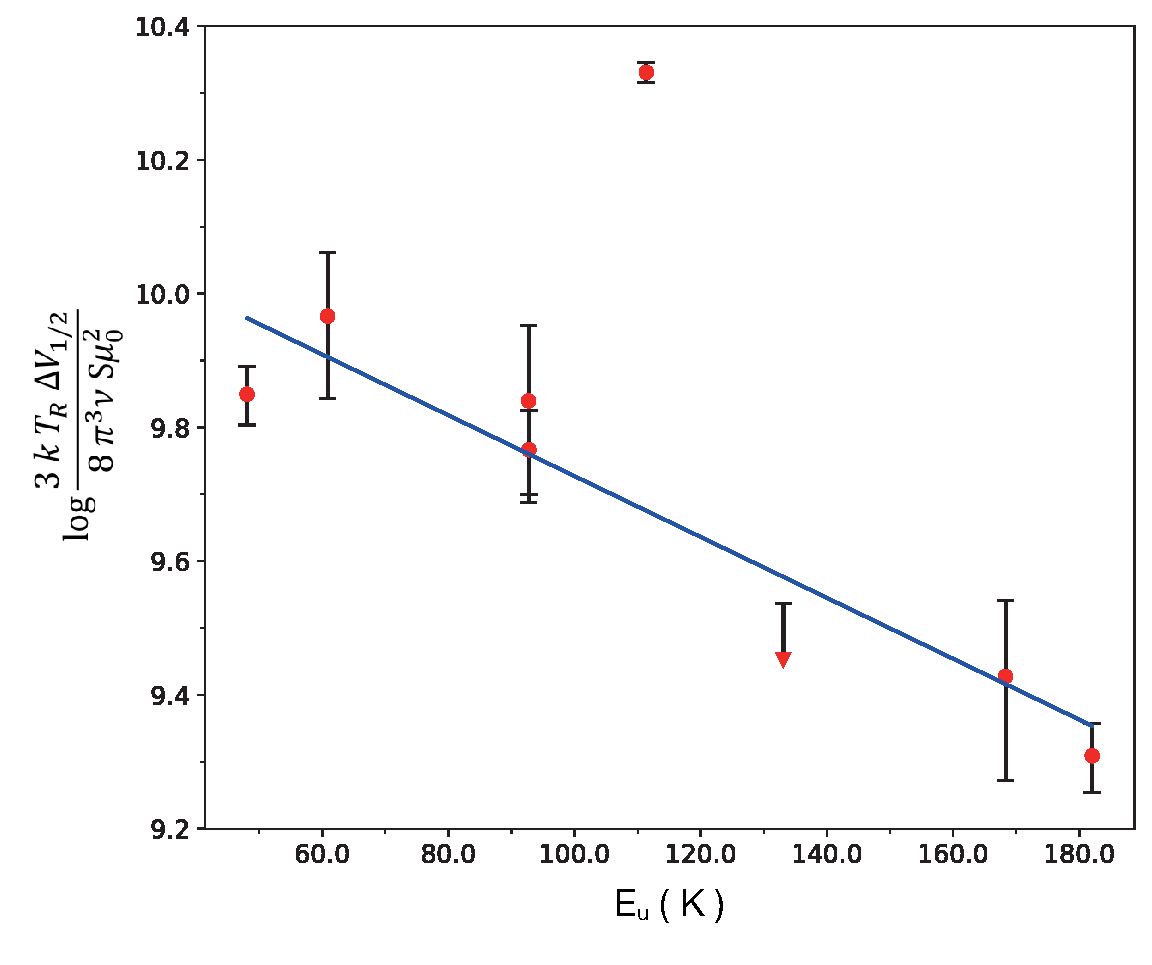
\includegraphics[width=0.7\textwidth]{OrionKL/RD_blend.eps}
  \caption{Rotation diagram of CH$_{3}$NH$_{2}$ in Hot core with additional 2 lines. The error bars on round plots represents $\pm$ 3$\sigma$ for each data. A signal below 3$\sigma$ is represented by a triangle with the error bar indicating the upper limit. The blue line is the same one as Figure \ref{fig:RD}.}
  \label{fig:RD_blend}
\end{figure}

\subsection*{215.670 GHz line}
This emission line ($E_{\mathrm{u}}=111$ K) is seen at Hot core and IRc7 like other CH$_{3}$NH$_{2}$ transitions 
(see Figure 4.3 and Figure \ref{ch_4}), but this line has stronger intensity than that predicted in the rotation diagram (see Figure \ref{fig:RD_blend}).
Since the line width is also wider than the other CH$_{3}$NH$_{2}$ transitions (see Figure 4.3), 
it appears that this line is blended with other molecular emission lines existing in Hot core.
Then examining the catalog including the transition of higher excitation, CH$_3$CH$_2$CN (215.6687 GHz, $E_{\mathrm{l}}$ = 604.845 K)
has come up as a candidate for blending.
However, considering that T$_{\mathrm{rot}}$ of CH$_3$CH$_2$CN in Hot core is 155 K \citep{Feng+2015}, 
it is uncertain how much this transition of higher excitation contributes to the blending.

\begin{figure}[htp] 
\begin{center}
\begin{minipage}{0.98\textwidth} 
\begin{center}
\begin{minipage}{0.48\textwidth}
\begin{center}
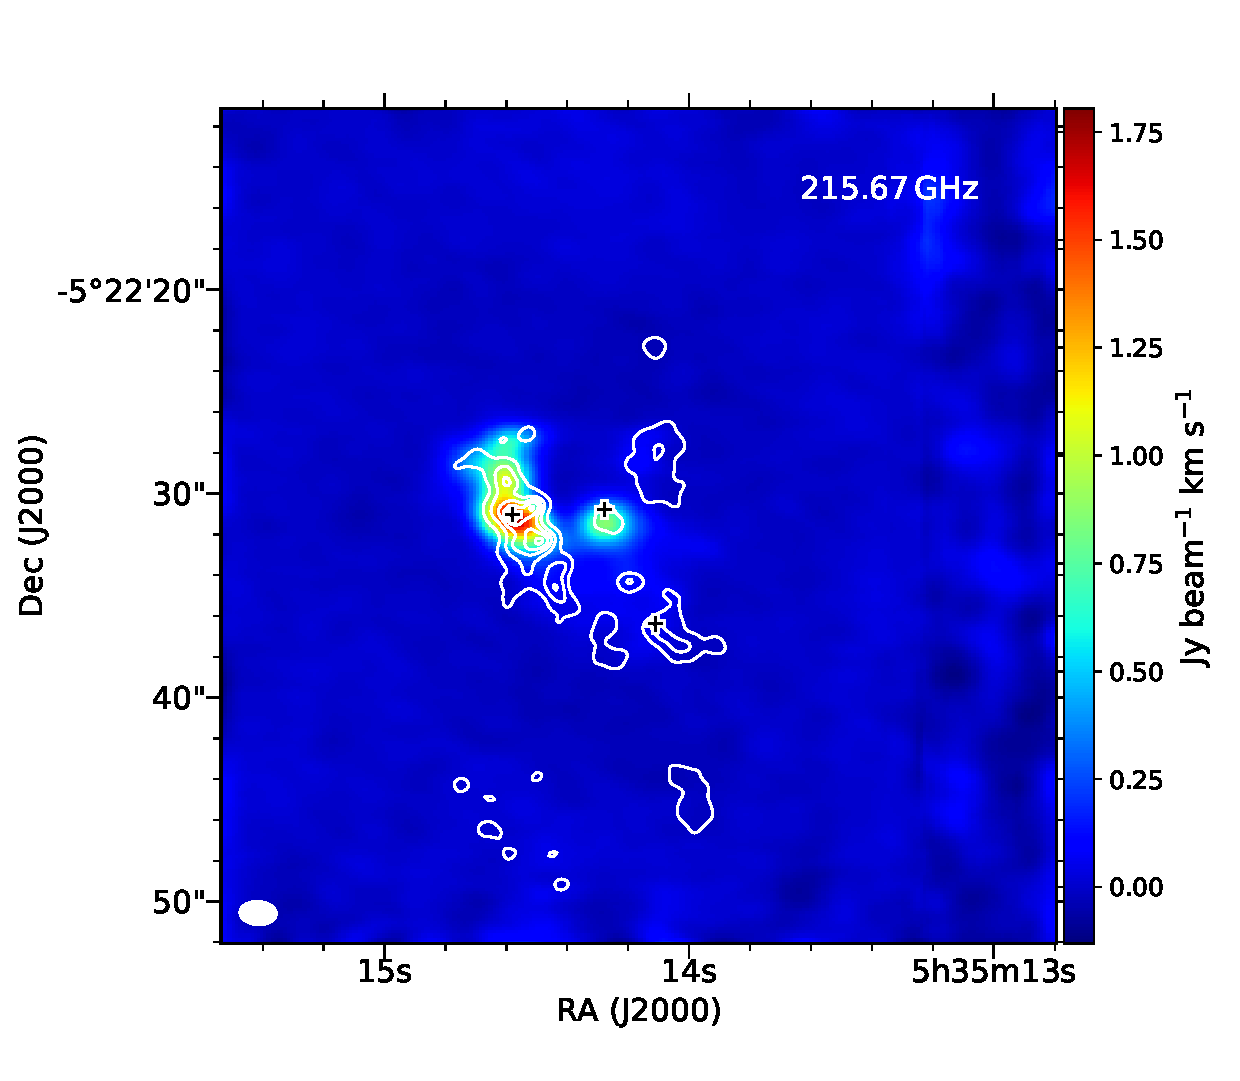
\includegraphics[width=0.98\textwidth]{OrionKL/mom0/215.67mom0_3-7.eps}
\end{center}
\end{minipage}
\begin{minipage}{0.48\textwidth}
\begin{center}
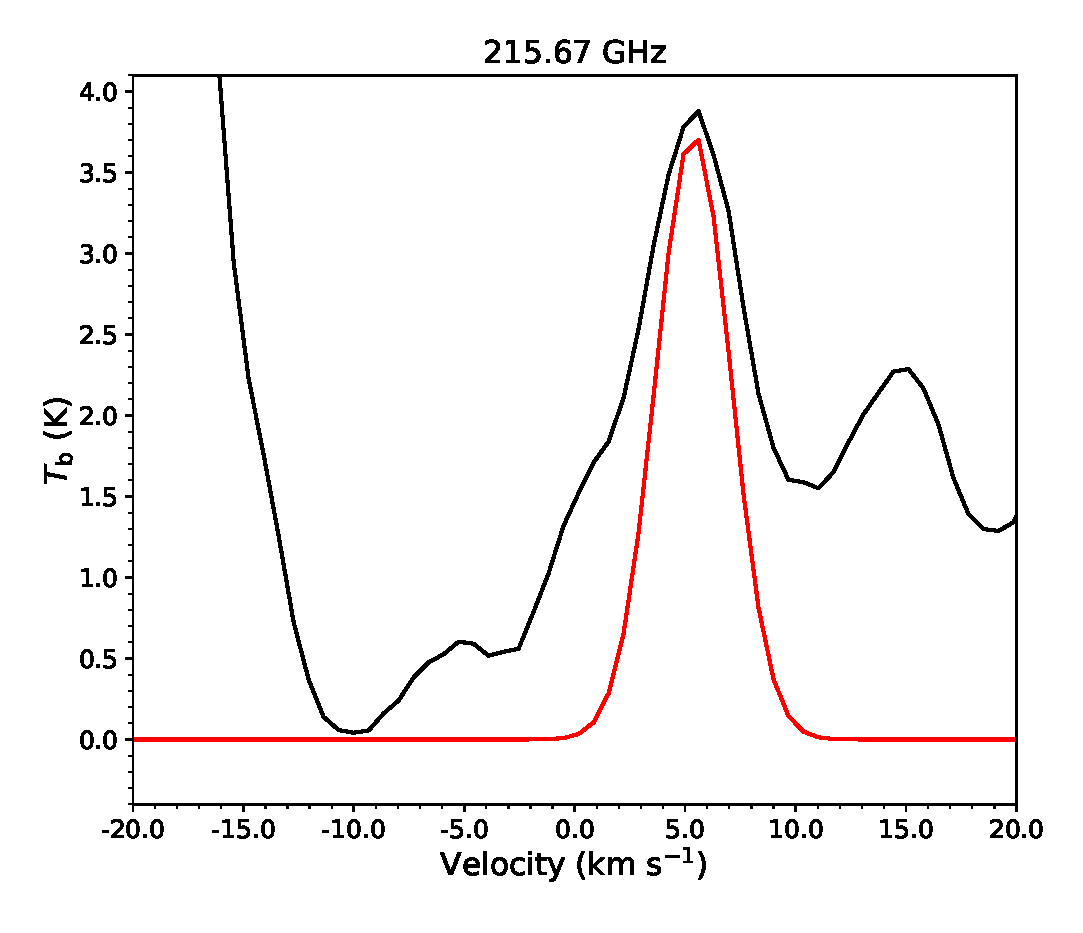
\includegraphics[width=0.98\textwidth]{OrionKL/spectrum/HC/215.6696452w_fit.eps}
\label{fig:215spec}
\end{center}
\end{minipage}
\end{center}
\end{minipage}
\label{fig:215data}
\caption{(left) Integrated intensity map of the emission for 215.670 GHz. Same as Figure \ref{fig:cont+2015} but for white contours and black crosses. (right) Spectrum of the CH$_3$NH$_2$ lines at each frequency observed in Hot core (black)  and the result of the Gaussian fitting assuming the average $\Delta V_{1/2} = 4.2\, \mathrm{km\,s^{-1}}$ (red)}
\end{center}
\label{fig:215data}
\end{figure}

\subsection*{221.755 GHz line}
A faint signal was seen in Hot core in the integrated intensity map and channel maps (Figure 4.4 and \ref{ch_6}).
Since there was no blend of other molecular emission lines in the comparison with the catalogs, we analyzed the spectrum, 
but the peak intensity ( $T_{\mathrm{B}}=$ 0.33 K) was weaker than 
3 $\sigma $ noise level ($T_{\mathrm{B}}=$ 0.133 K, see Table \ref{tab:unresolved}). 
When we plotted this line on the rotation diagram with 3$\sigma$ as the upper limit of the intensity, 
the derived value was consistent with other CH$_3$NH$_2$ transitions (see Figure \ref{fig:RD_blend}). 
This emission line was included in SV data cube, 
so it could be possible to detect the line in future observations with higher S/N ratio.

\begin{figure}[htp] 
\begin{center}
\begin{minipage}{0.98\textwidth} 
\begin{center}
\begin{minipage}{0.48\textwidth}
\begin{center}
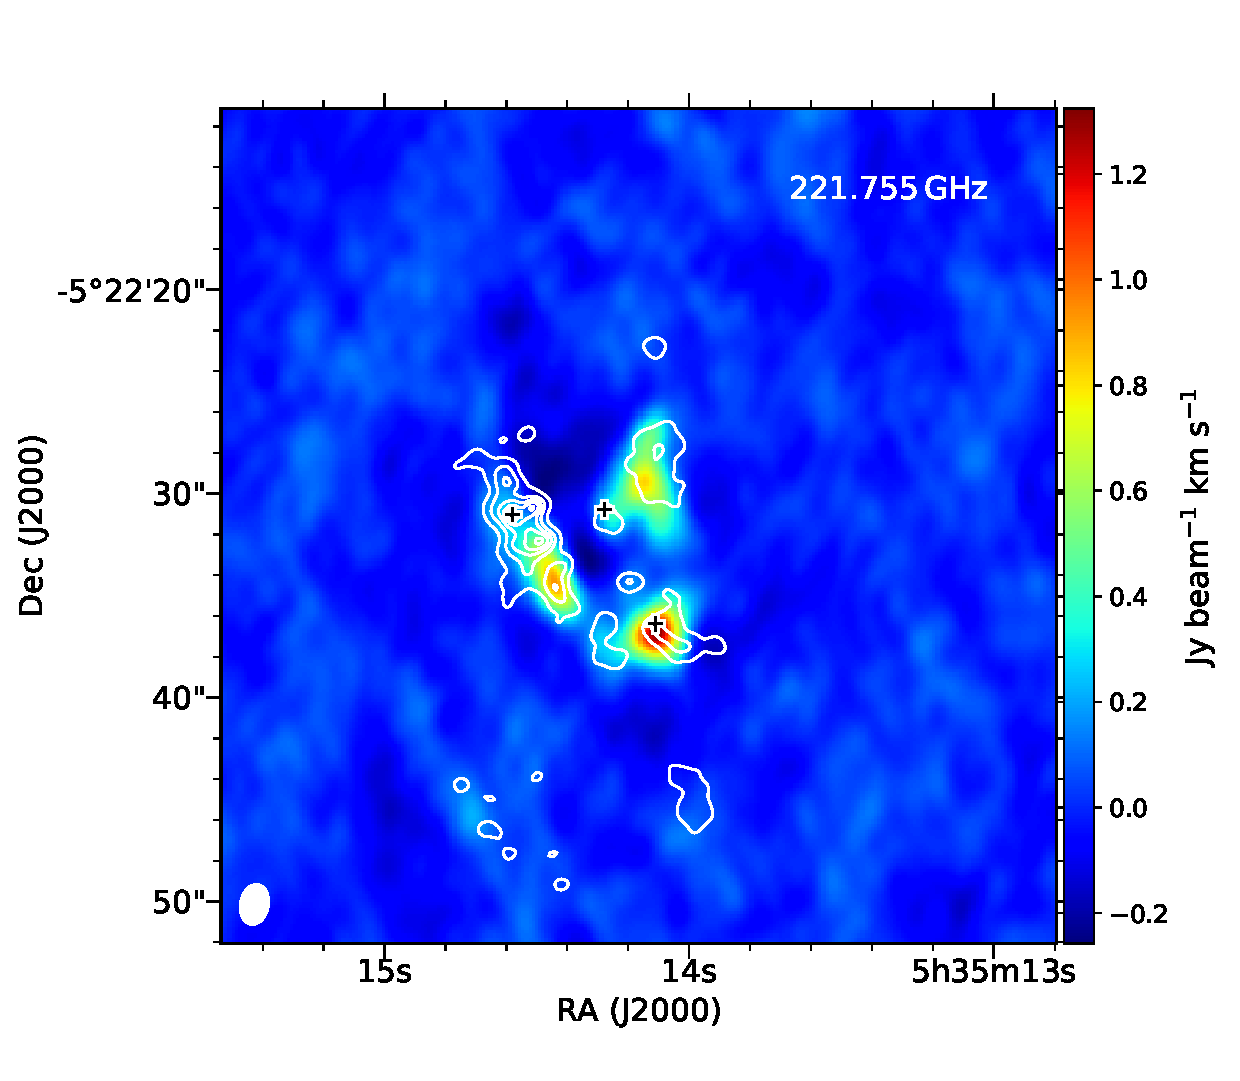
\includegraphics[width=0.98\textwidth]{OrionKL/mom0/221.755SV_mom0_3-7.eps}
\label{fig:221mom}
\end{center}
\end{minipage}
\begin{minipage}{0.48\textwidth}
\begin{center}
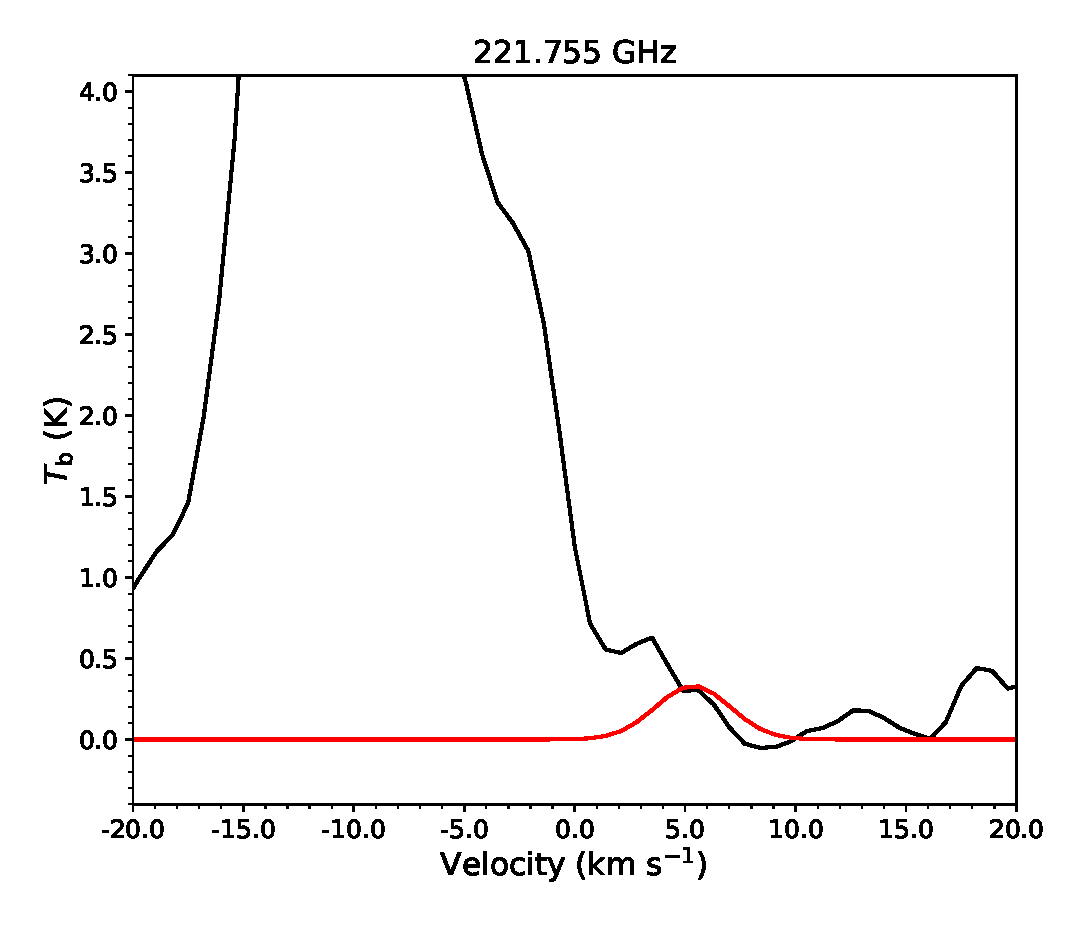
\includegraphics[width=0.98\textwidth]{OrionKL/spectrum/HC/221.755055w_fit.eps}
\end{center}
\end{minipage}
\end{center}
\end{minipage}
\caption{(left) Integrated intensity map of the emission for 221.755 GHz. Same as Figure \ref{fig:cont+2015} but for white contours and black crosses. (right) Spectrum of the CH$_3$NH$_2$ lines at each frequency observed in Hot core (black)  and the result of the Gaussian fitting assuming the average $\Delta V_{1/2} = 4.2\, \mathrm{km\,s^{-1}}$ (red)}
\end{center}
\end{figure}

\begin{figure}[htp]
  \centering
  \includegraphics[width=0.98\textwidth]{OrionKL/chmap/215.67.eps}
  \caption{Channel map around 215.670 GHz. Same as Figure \ref{ch_0} but for white contours and mazenta crosses.}
  \label{ch_4}
\end{figure}

\begin{figure}[htp]
  \centering
  \includegraphics[width=0.98\textwidth]{OrionKL/chmap/221.755.eps}
  \caption{Channel map around 221.755 GHz line. Same as Figure \ref{ch_0} but for white contours and mazenta crosses.}
  \label{ch_6}
\end{figure}

%\thispagestyle{empty}\mbox{}\newpage
\chapter{Summary
  \label{chap:}}

%\thispagestyle{empty}\mbox{}\newpage

%%% appendix %%%
\appendix
\chapter{Distribution of methylamine lines contaminated by other molecular line emission in Orion-KL
\label{chap:appendixA}}

\section{Integrated intensity maps}

%%%%% 積分強度図挿入 %%%%%
\begin{figure}[htbp] 
\begin{center}
\begin{minipage}{0.98\textwidth} 
\begin{center}
%%%% ここから
\begin{minipage}{0.48\textwidth}
\begin{center}
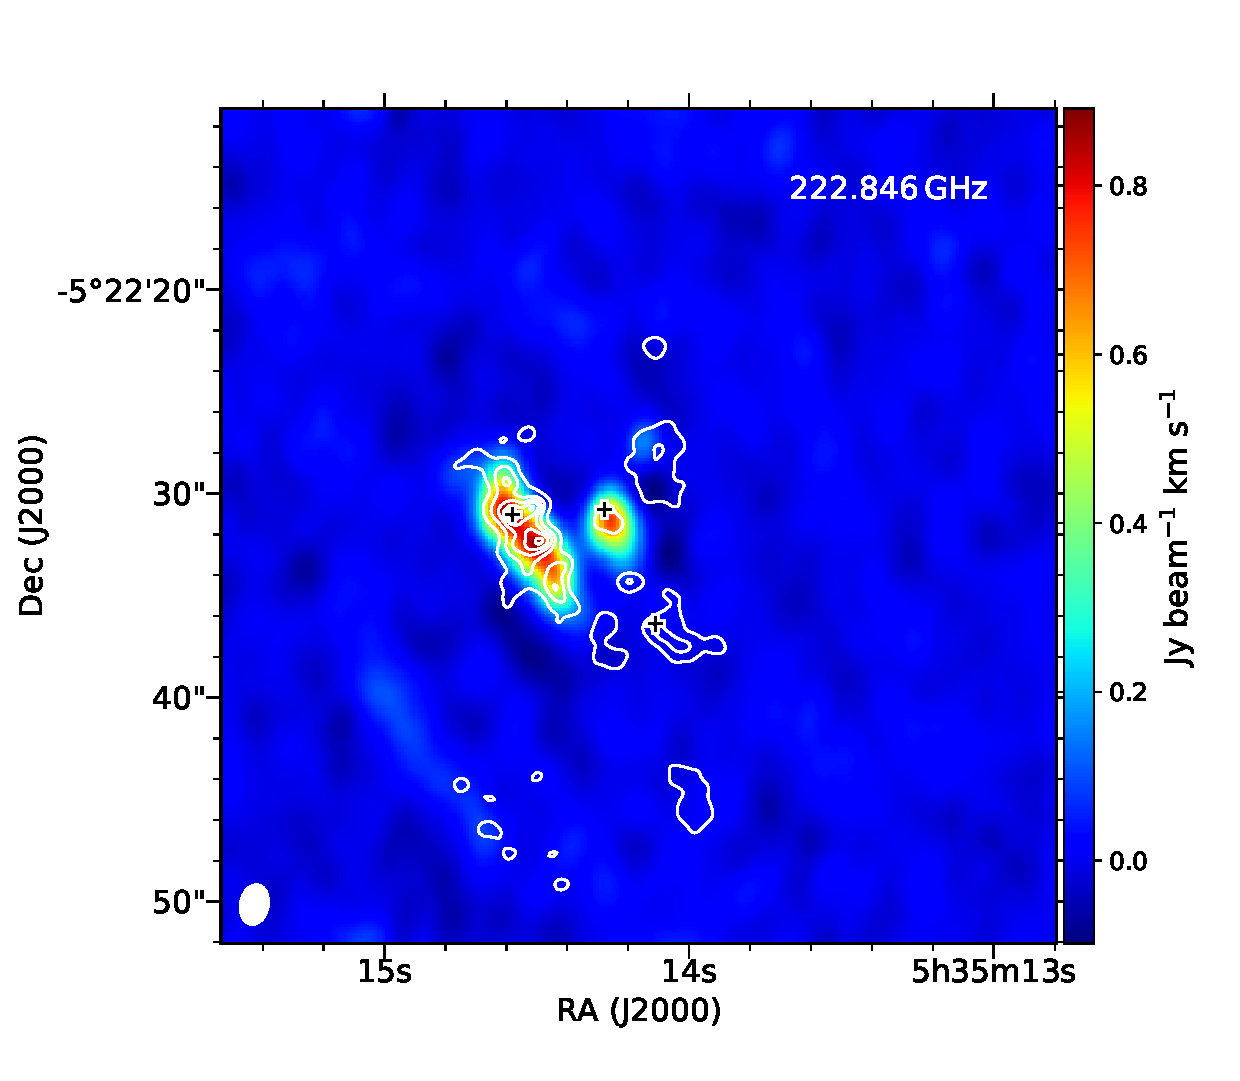
\includegraphics[width=0.98\textwidth]{OrionKL/mom0/222.846SV_mom0_3-7.eps}
%\\(a) 左の図の説明
\end{center}
\end{minipage}
\begin{minipage}{0.48\textwidth}
\begin{center}
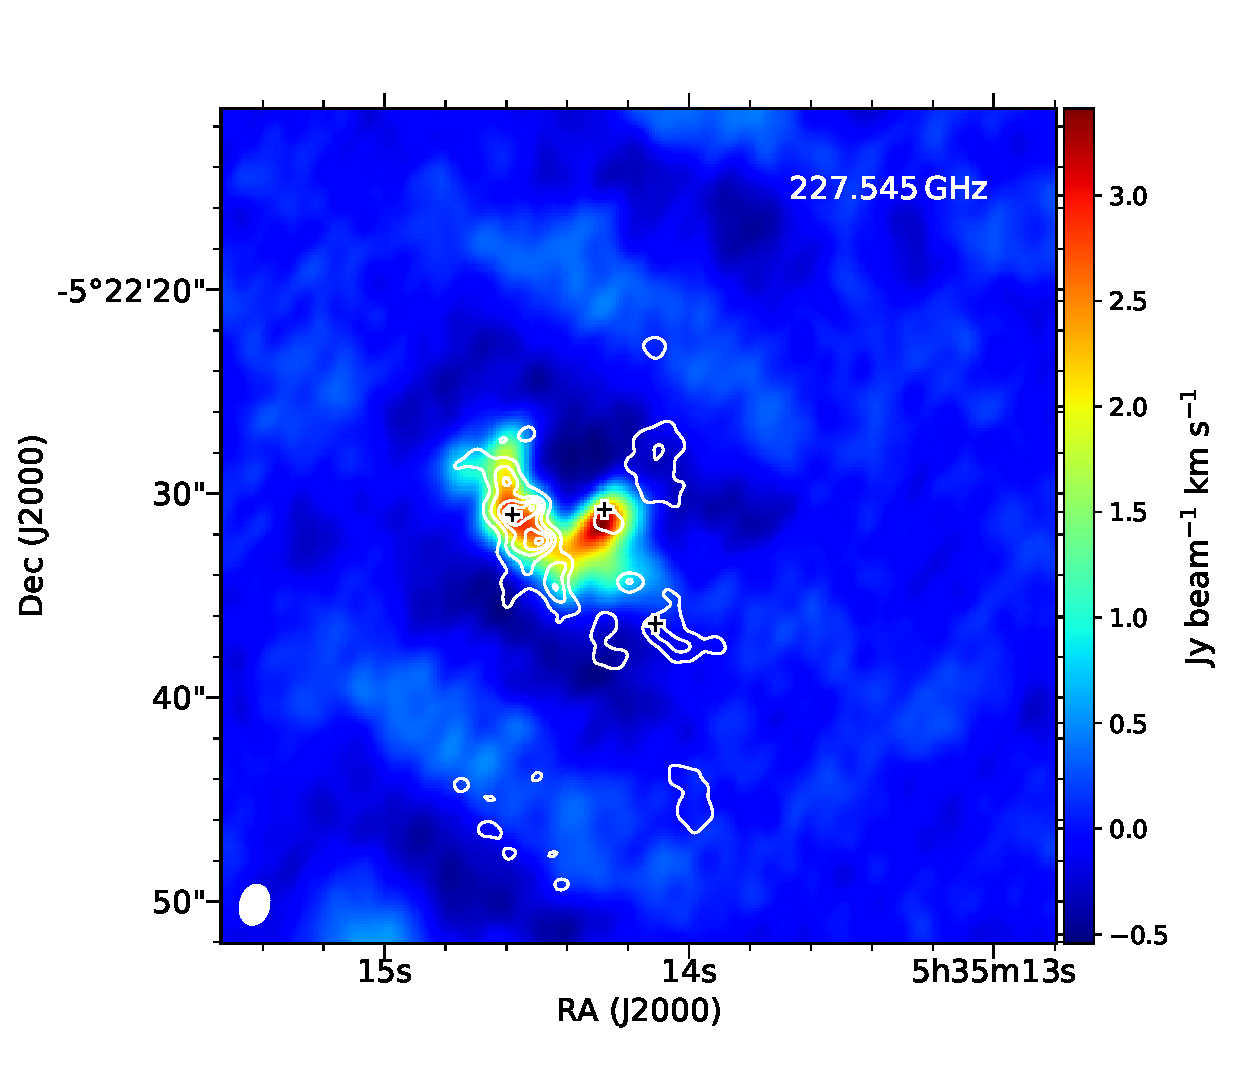
\includegraphics[width=0.98\textwidth]{OrionKL/mom0/227.545SV_mom0_3-7.eps}
%\\(b) 右の図の説明
\end{center}
\end{minipage}
\end{center}
\end{minipage}
%%%% ここまで一組

\begin{minipage}{0.98\textwidth} 
\begin{center}
\begin{minipage}{0.48\textwidth}
\begin{center}
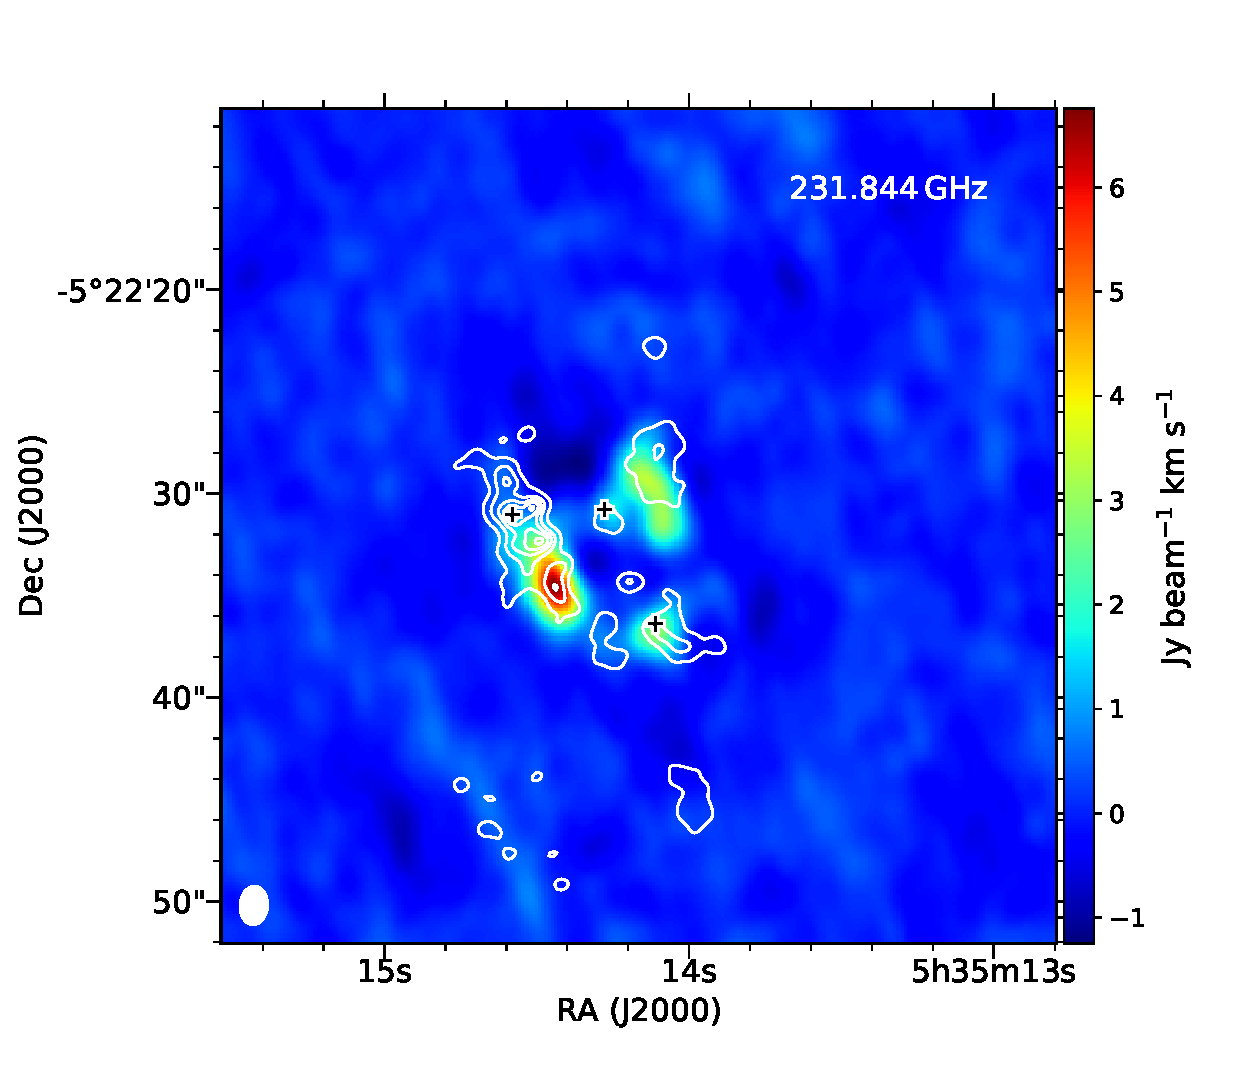
\includegraphics[width=0.98\textwidth]{OrionKL/mom0/231.844SV_mom0_3-7.eps}
%\\(c) 左の図の説明
\end{center}
\end{minipage}
\begin{minipage}{0.48\textwidth}
\begin{center}
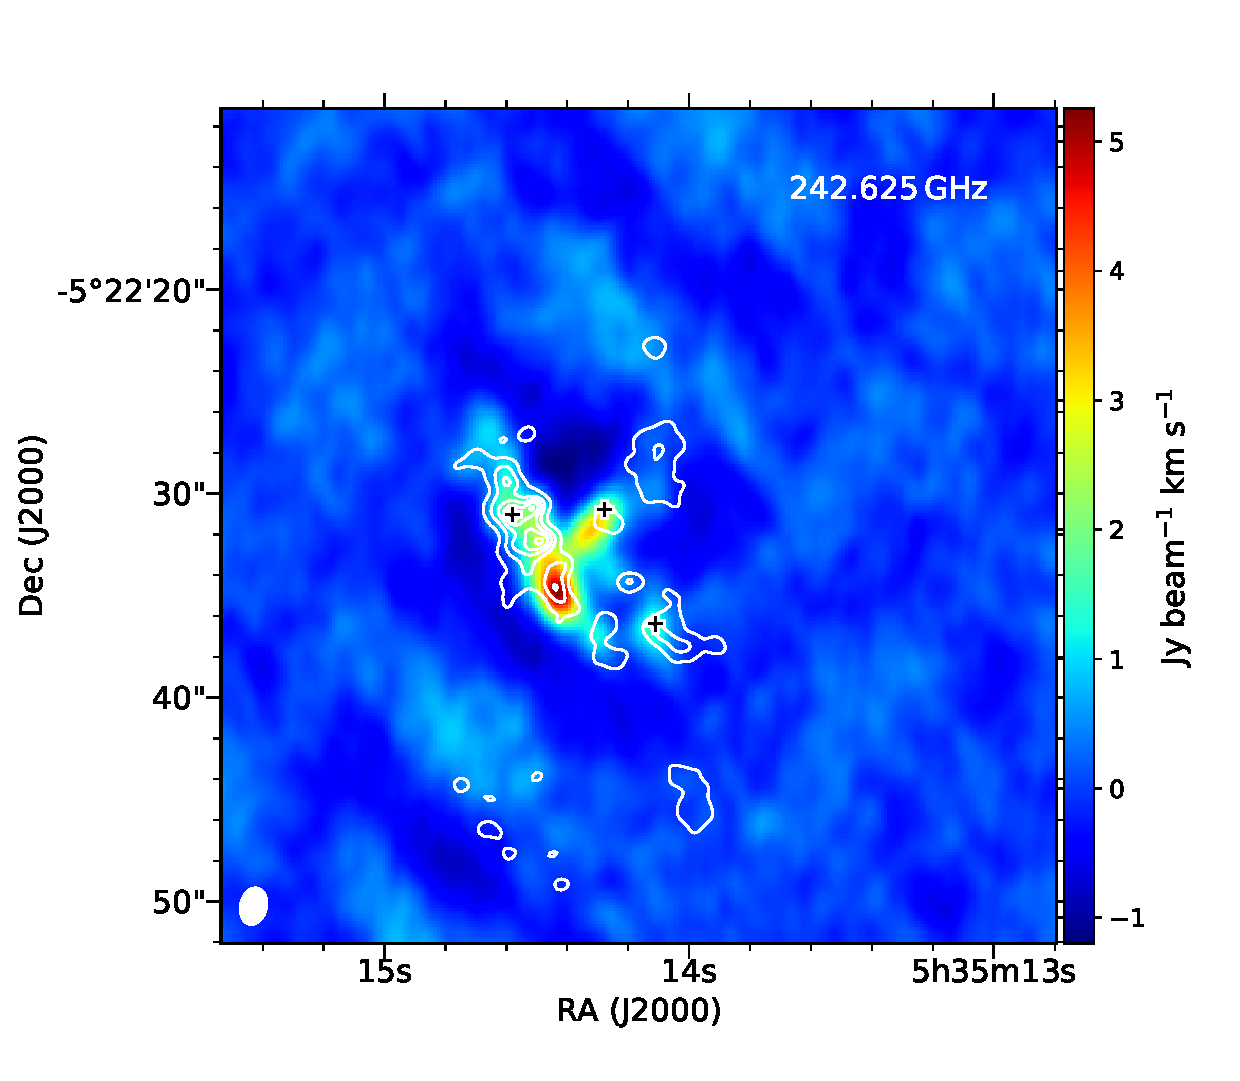
\includegraphics[width=0.98\textwidth]{OrionKL/mom0/242.625SV_mom0_3-7.eps}
%\\(d) 右の図の説明
\end{center}
\end{minipage}
\end{center}
\end{minipage}

\caption{Integrated intensity maps around methylamine line.}
\end{center}
\end{figure}

\newpage

%%%%% 積分強度図挿入 %%%%%
\begin{figure}[H] 
\begin{center}

%%%% ここから
\begin{minipage}{0.98\textwidth} 
\begin{center}
\begin{minipage}{0.48\textwidth}
\begin{center}
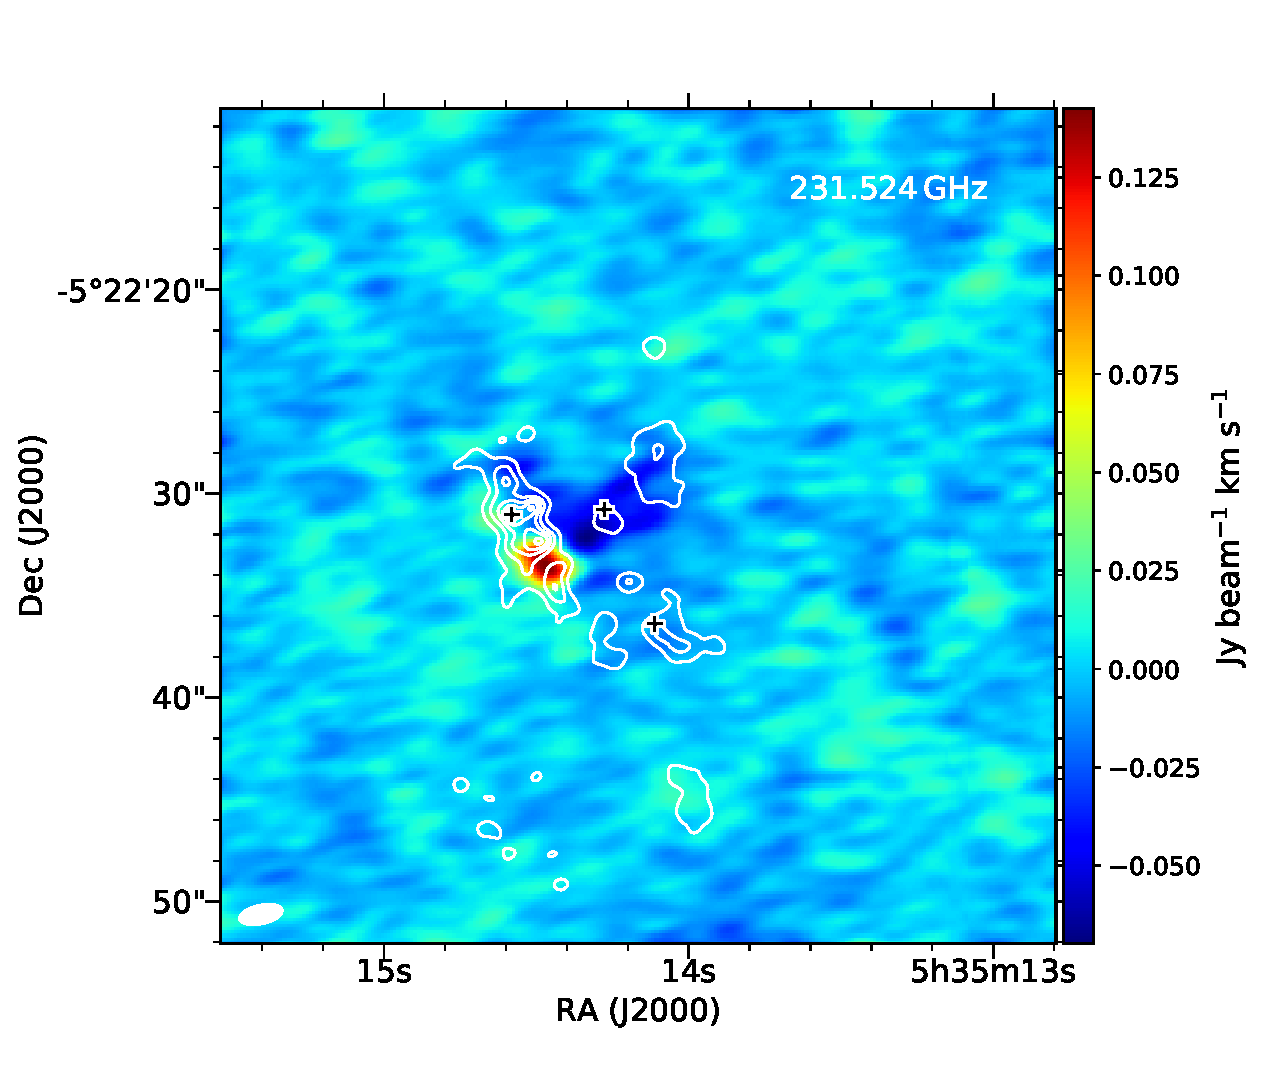
\includegraphics[width=0.98\textwidth]{OrionKL/mom0/231.524mom0_3-7.eps}
%\\(a) 左の図の説明
\end{center}
\end{minipage}
\begin{minipage}{0.48\textwidth}
\begin{center}
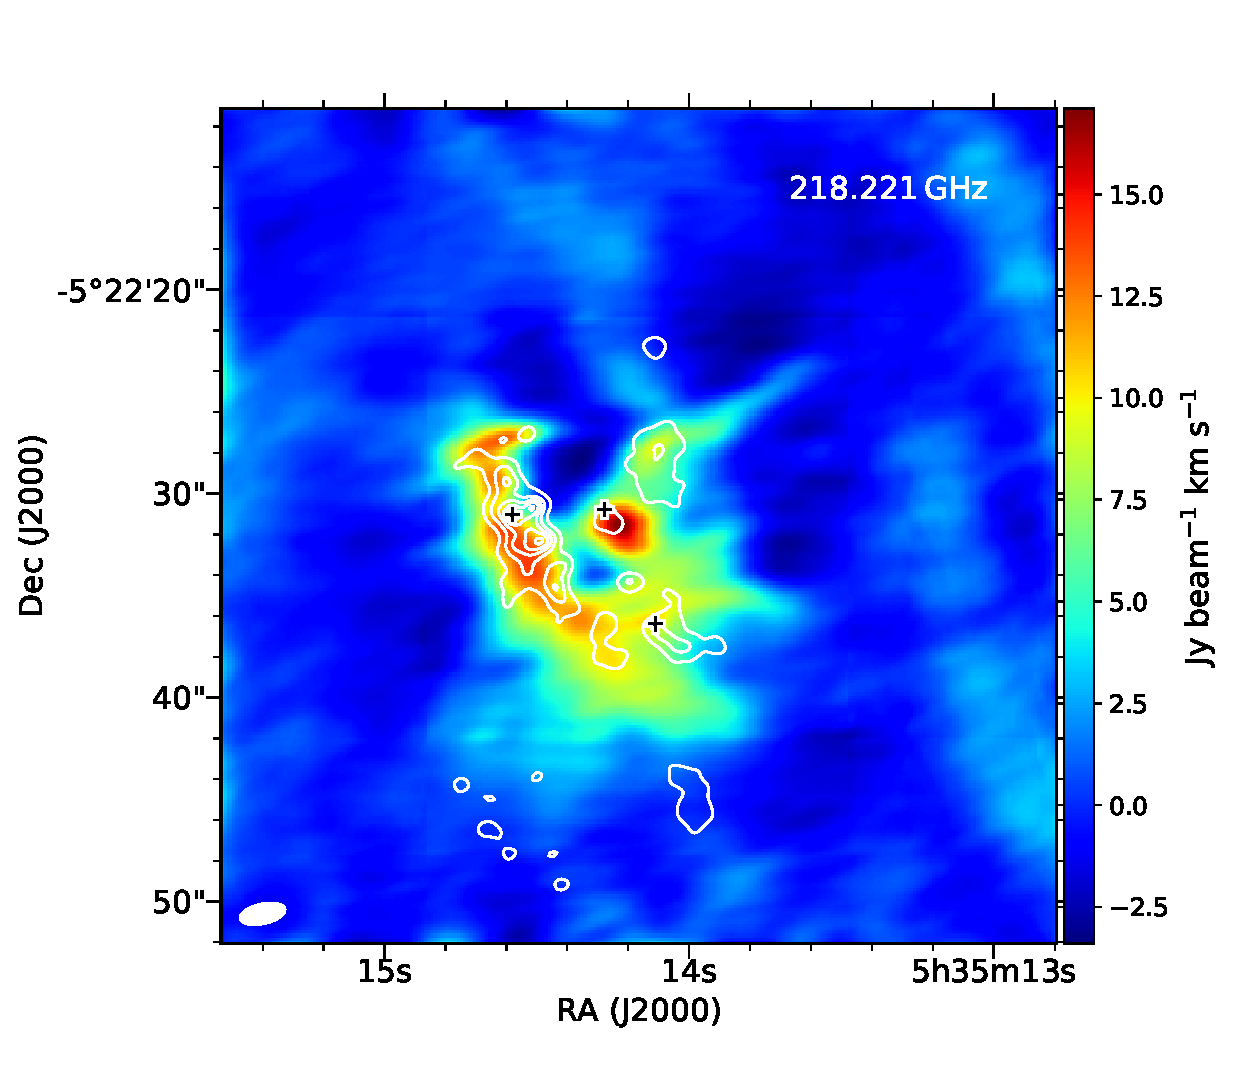
\includegraphics[width=0.98\textwidth]{OrionKL/mom0/218.221mom0_3-7.eps}
%\\(b) 右の図の説明
\end{center}
\end{minipage}
\end{center}
\end{minipage}
%%%% ここまで一組

\begin{minipage}{0.98\textwidth} 
\begin{center}
\begin{minipage}{0.48\textwidth}
\begin{center}
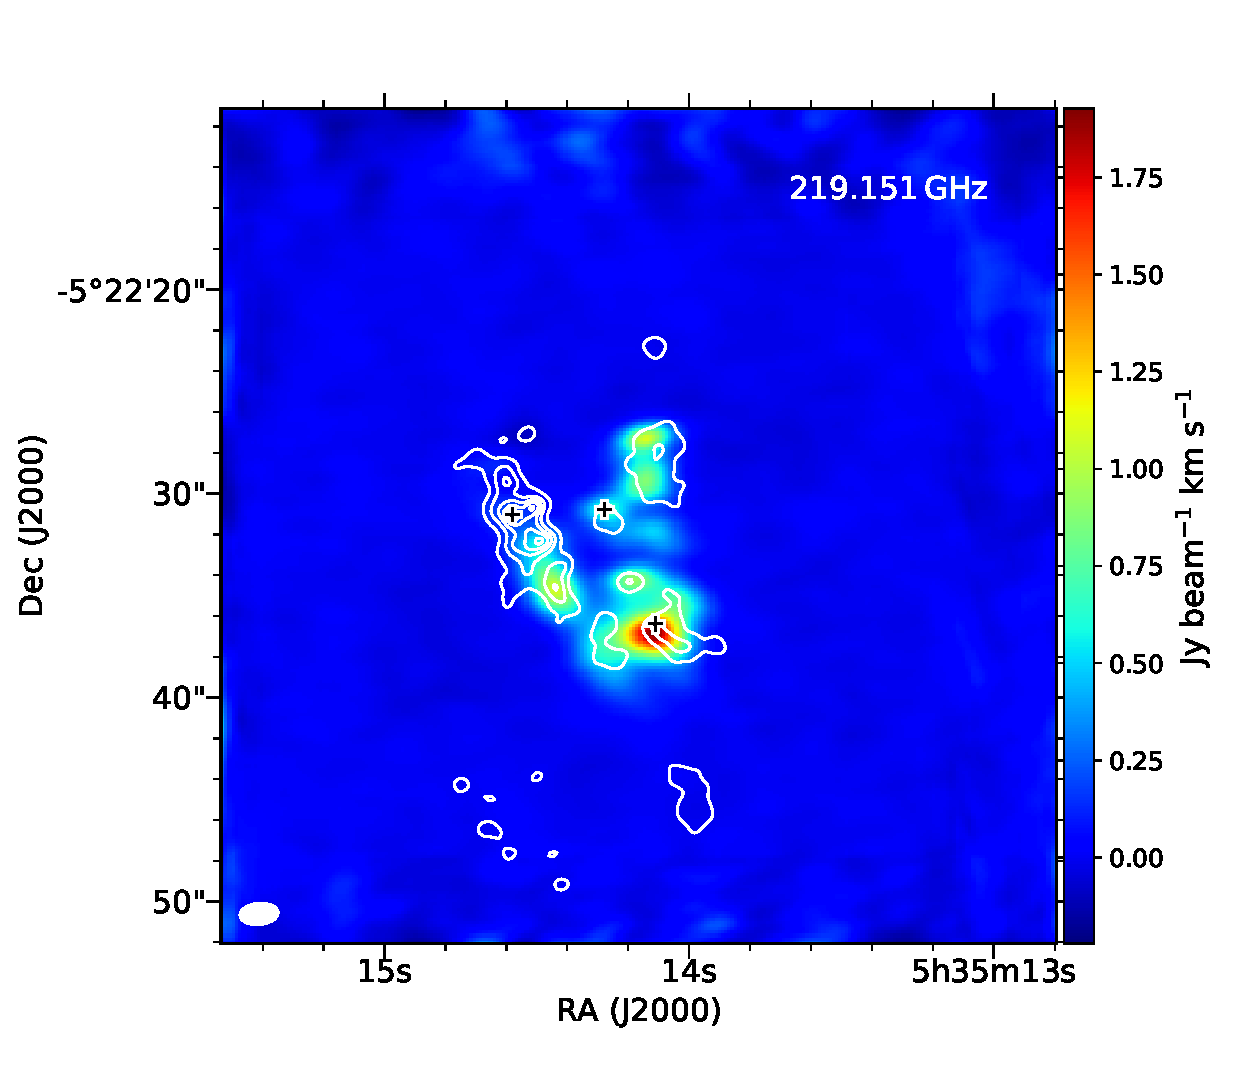
\includegraphics[width=0.98\textwidth]{OrionKL/mom0/219.151mom0_3-7.eps}
%\\(c) 左の図の説明
\end{center}
\end{minipage}
\begin{minipage}{0.48\textwidth}
\begin{center}
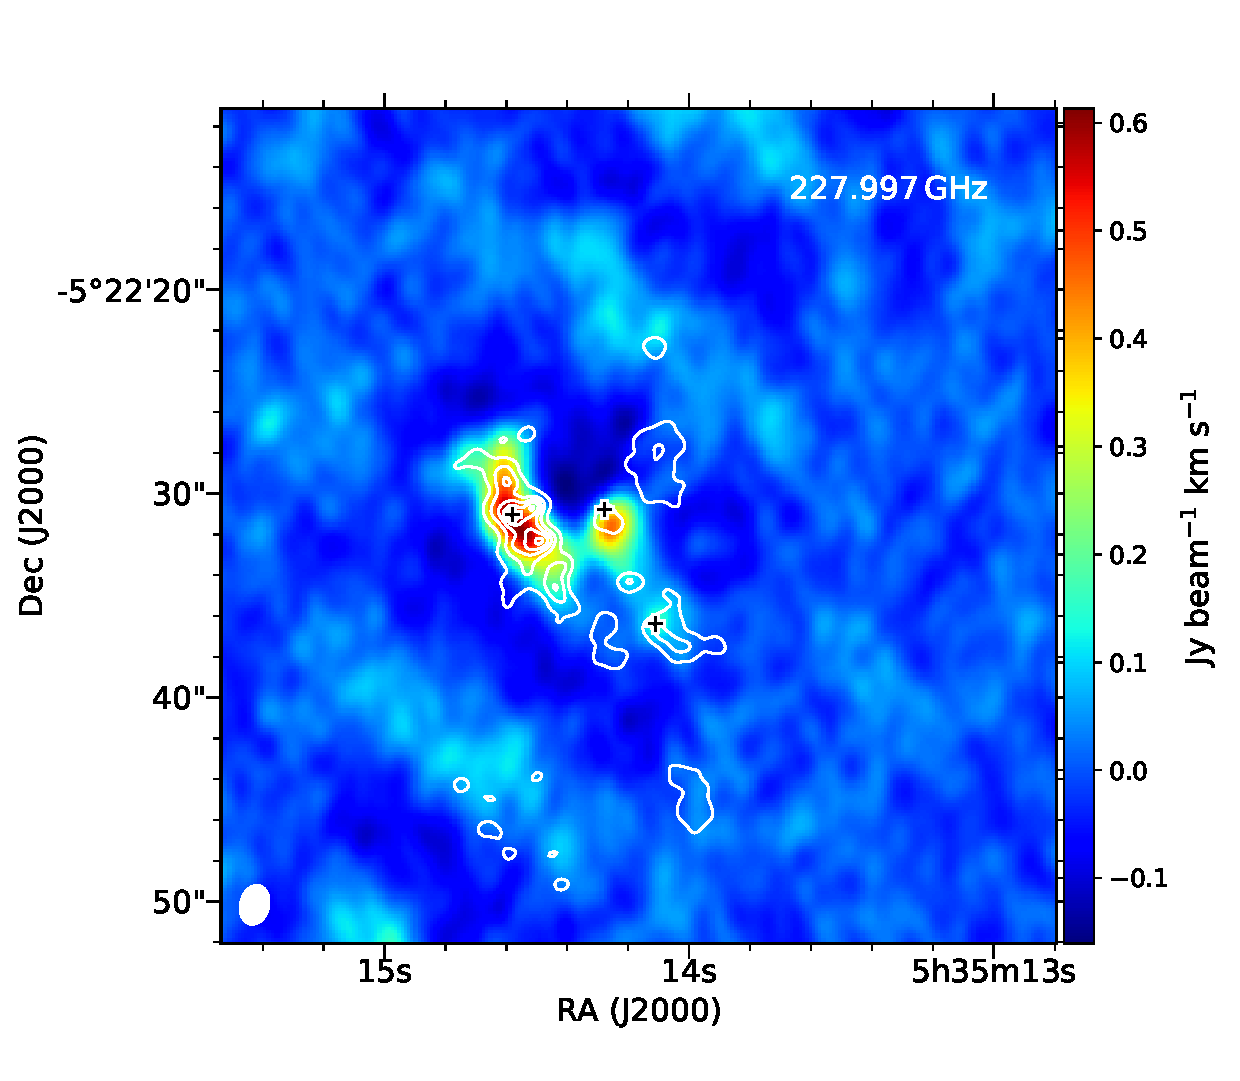
\includegraphics[width=0.98\textwidth]{OrionKL/mom0/227.997SV_mom0_3-7.eps}
%\\(d) 右の図の説明
\end{center}
\end{minipage}
\end{center}
\end{minipage}

%%%% ここから
\begin{minipage}{0.98\textwidth} 
\begin{center}
\begin{minipage}{0.48\textwidth}
\begin{center}
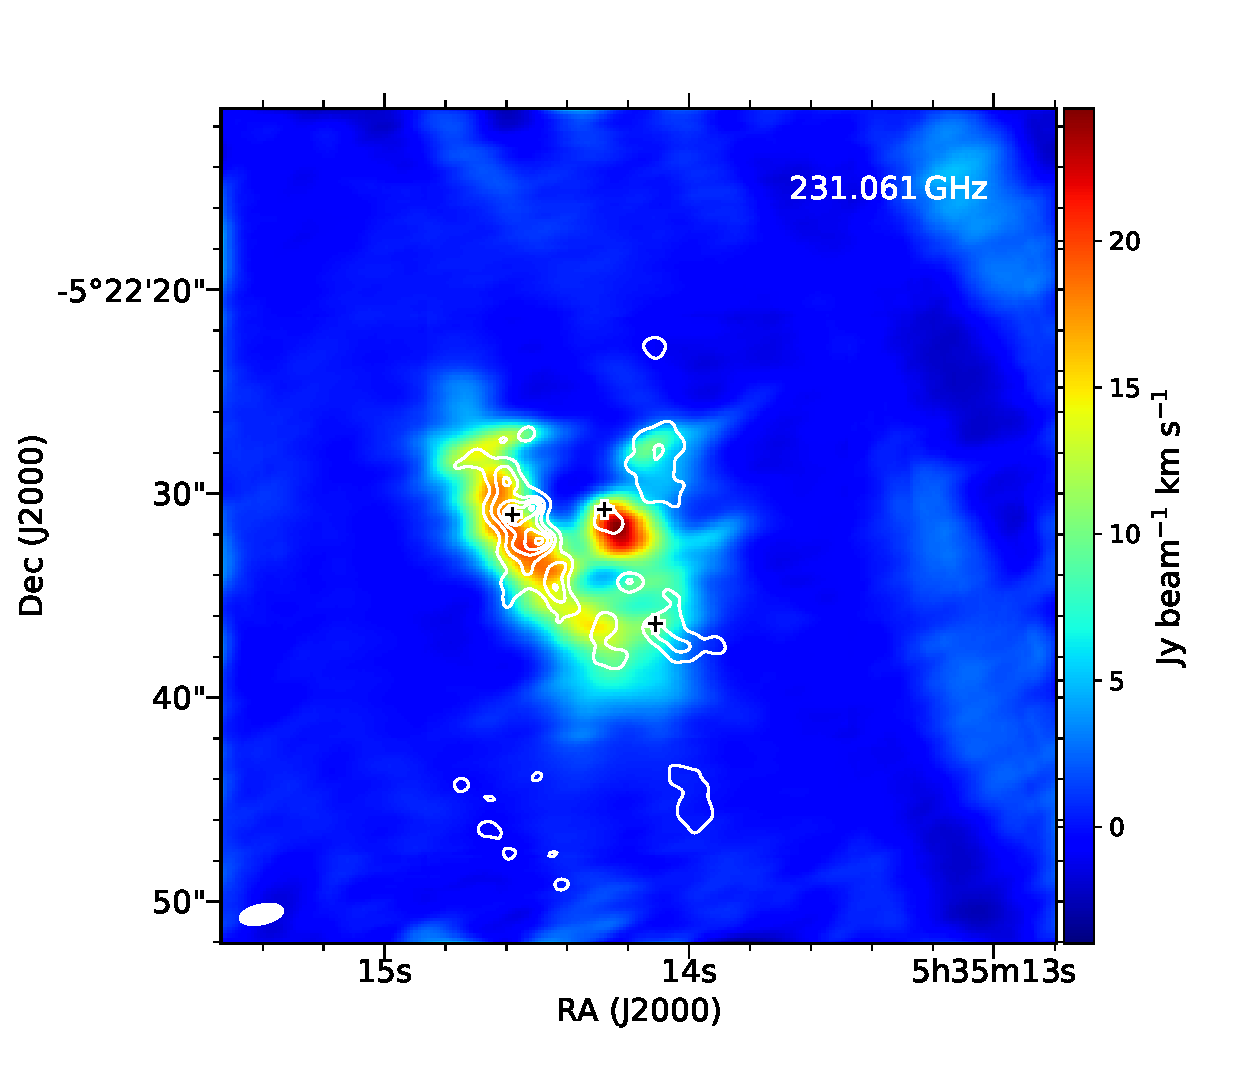
\includegraphics[width=0.98\textwidth]{OrionKL/mom0/231.061mom0_3-7.eps}
%\\(e) 左の図の説明
\end{center}
\end{minipage}
\begin{minipage}{0.48\textwidth}
\begin{center}
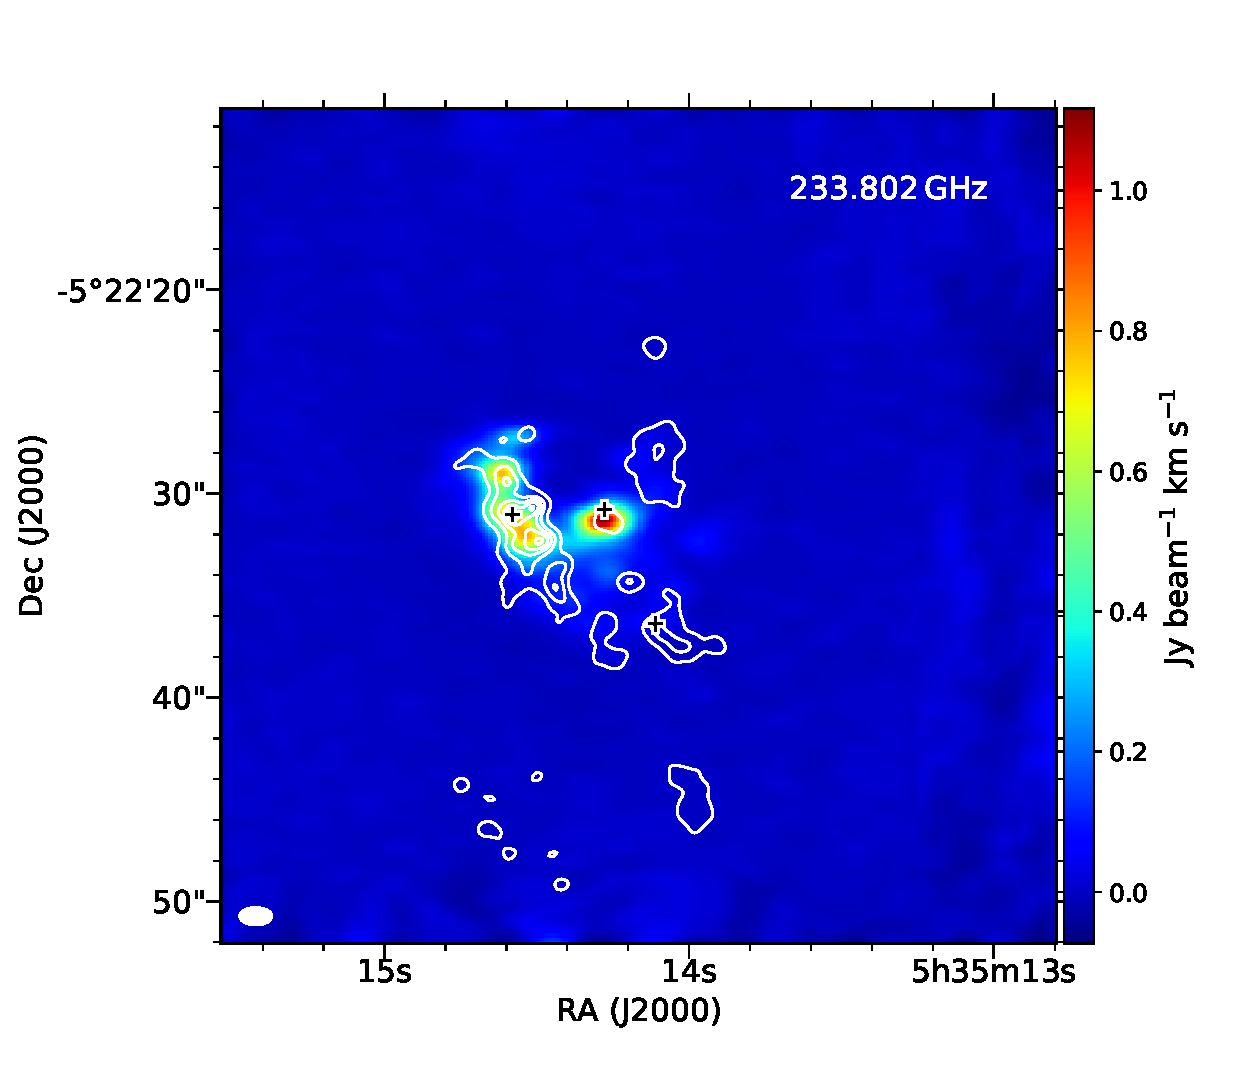
\includegraphics[width=0.98\textwidth]{OrionKL/mom0/233.802mom0_3-7.eps}
%\\(f) 右の図の説明
\end{center}
\end{minipage}
\end{center}
\end{minipage}
%%%% ここまで一組

\caption{(Continued)}
\end{center}
\end{figure}
%%%%%% ここまで

\newpage

%%%%% 積分強度図挿入 %%%%%
\begin{figure}[H] 
\begin{center}

%%%% ここから
\begin{minipage}{0.98\textwidth} 
\begin{center}
\begin{minipage}{0.48\textwidth}
\begin{center}
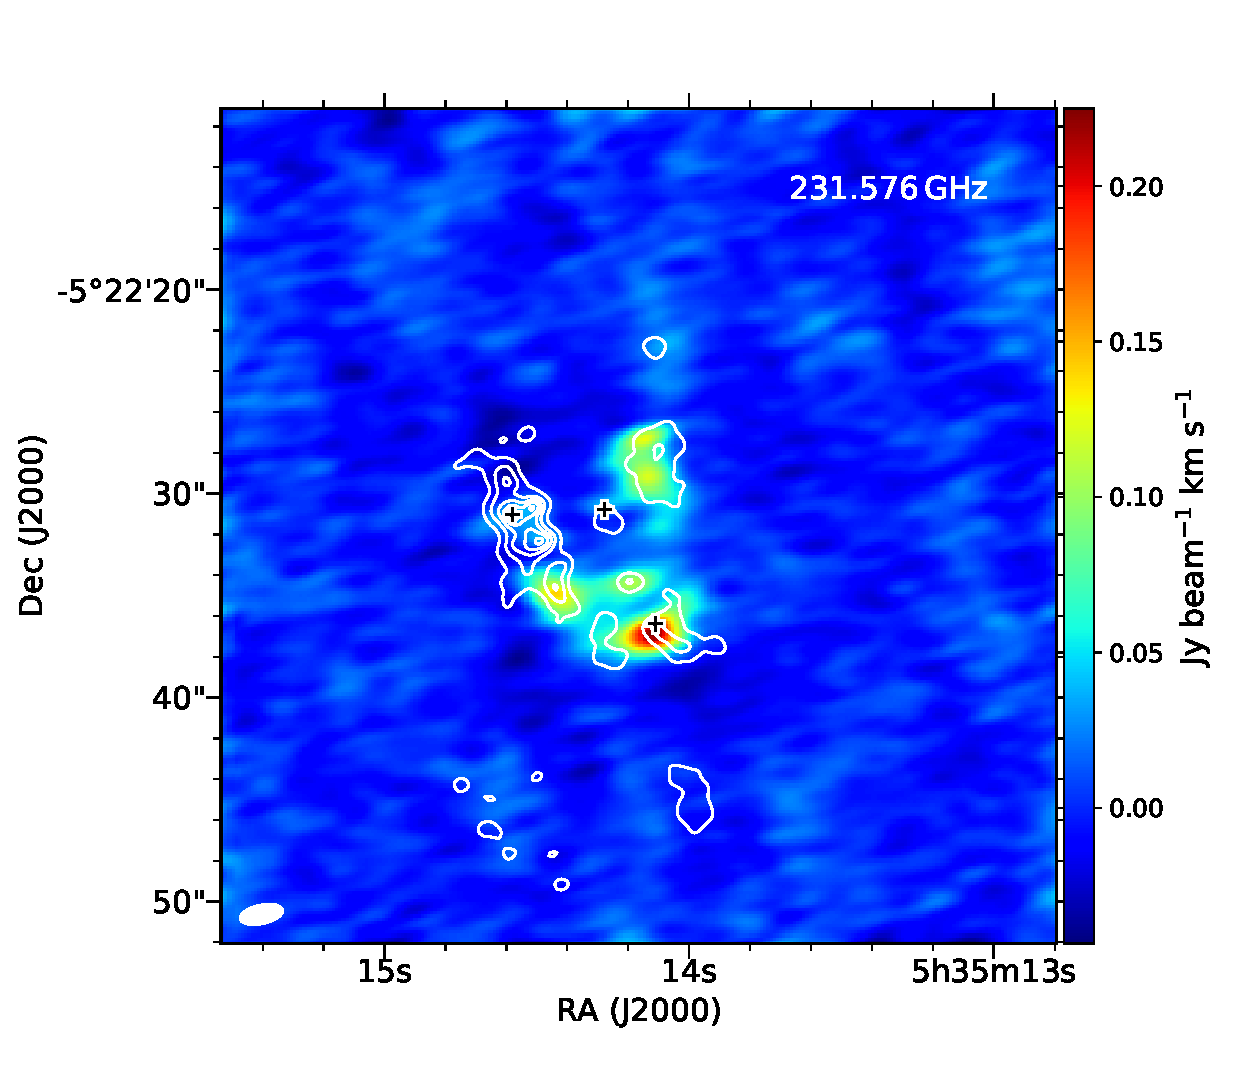
\includegraphics[width=0.98\textwidth]{OrionKL/mom0/231.576mom0_3-7.eps}
%\\(a) 左の図の説明
\end{center}
\end{minipage}
\begin{minipage}{0.48\textwidth}
\begin{center}
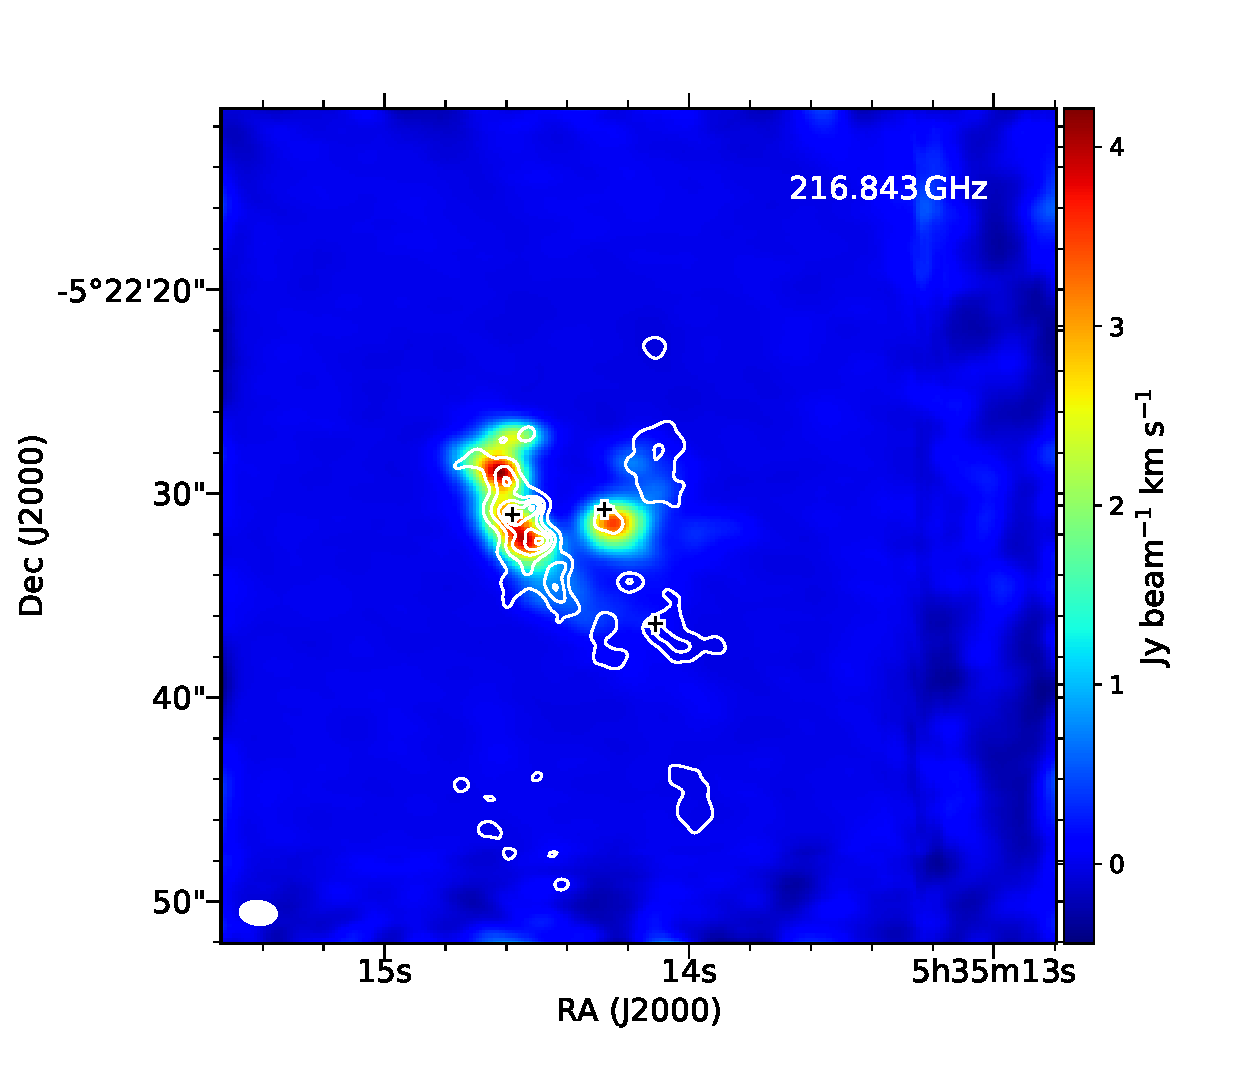
\includegraphics[width=0.98\textwidth]{OrionKL/mom0/216.843mom0_3-7.eps}
%\\(b) 右の図の説明
\end{center}
\end{minipage}
\end{center}
\end{minipage}
%%%% ここまで一組

\begin{minipage}{0.98\textwidth} 
\begin{center}
\begin{minipage}{0.48\textwidth}
\begin{center}
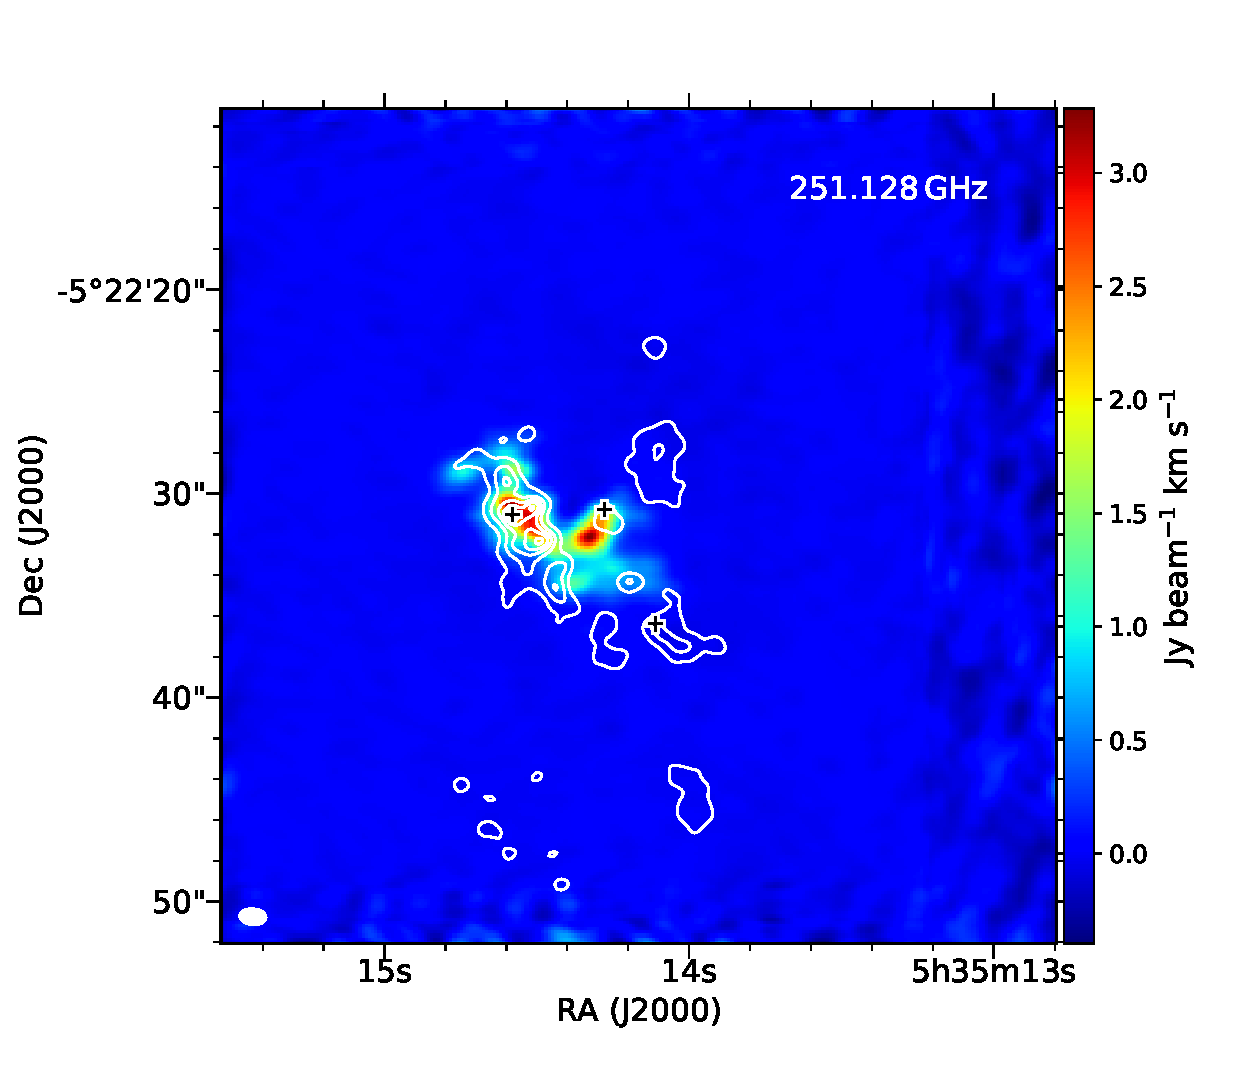
\includegraphics[width=0.98\textwidth]{OrionKL/mom0/251.128mom0_3-7.eps}
%\\(c) 左の図の説明
\end{center}
\end{minipage}
\begin{minipage}{0.48\textwidth}
\begin{center}
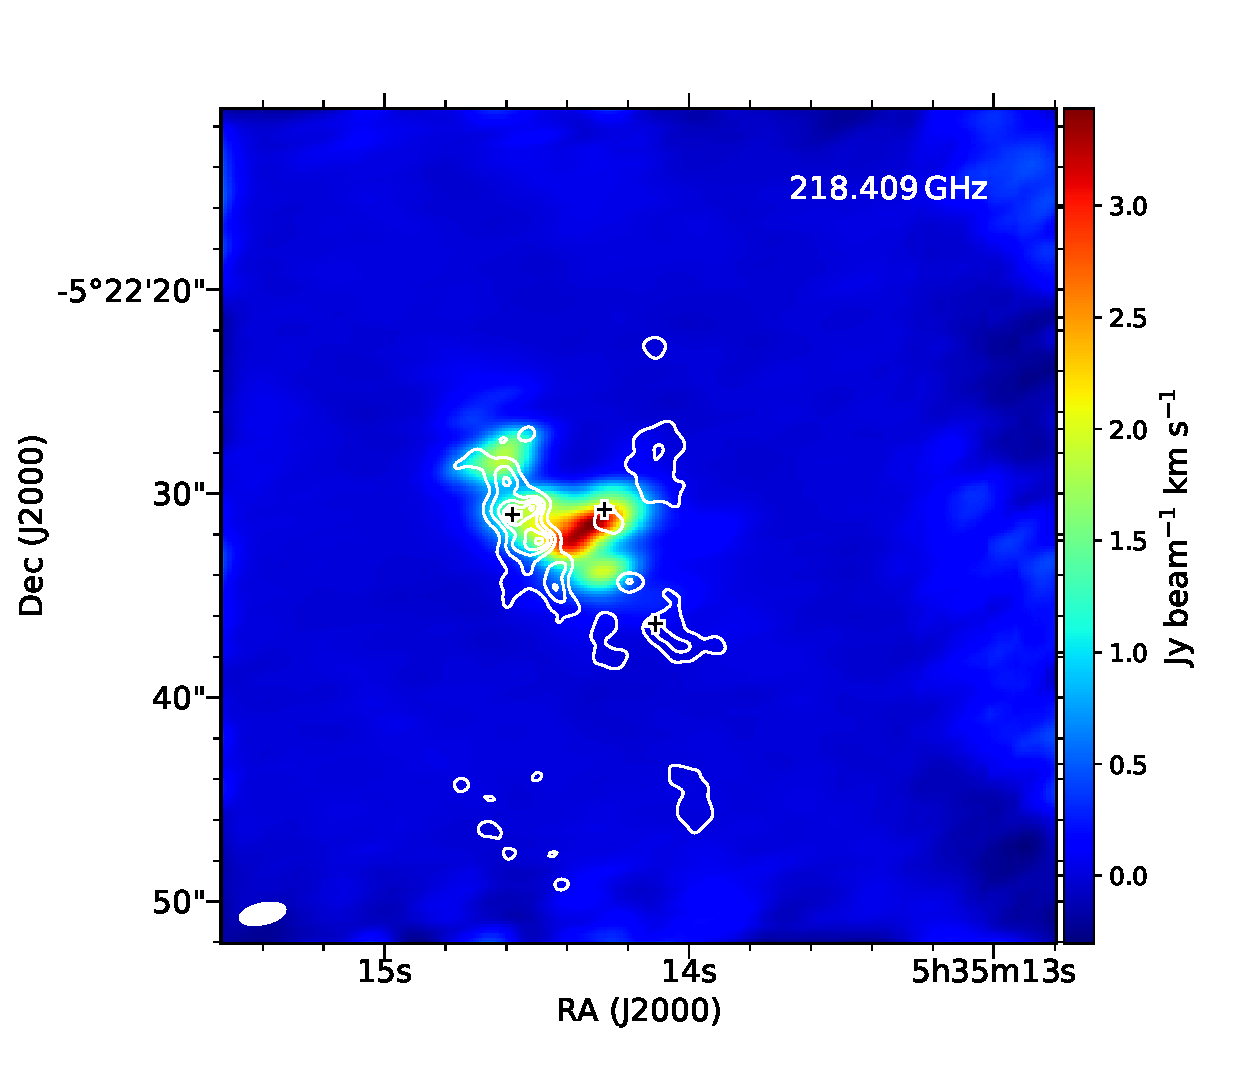
\includegraphics[width=0.98\textwidth]{OrionKL/mom0/218.409mom0_3-7.eps}
%\\(d) 右の図の説明
\end{center}
\end{minipage}
\end{center}
\end{minipage}

%%%% ここから
\begin{minipage}{0.98\textwidth} 
\begin{center}
\begin{minipage}{0.48\textwidth}
\begin{center}
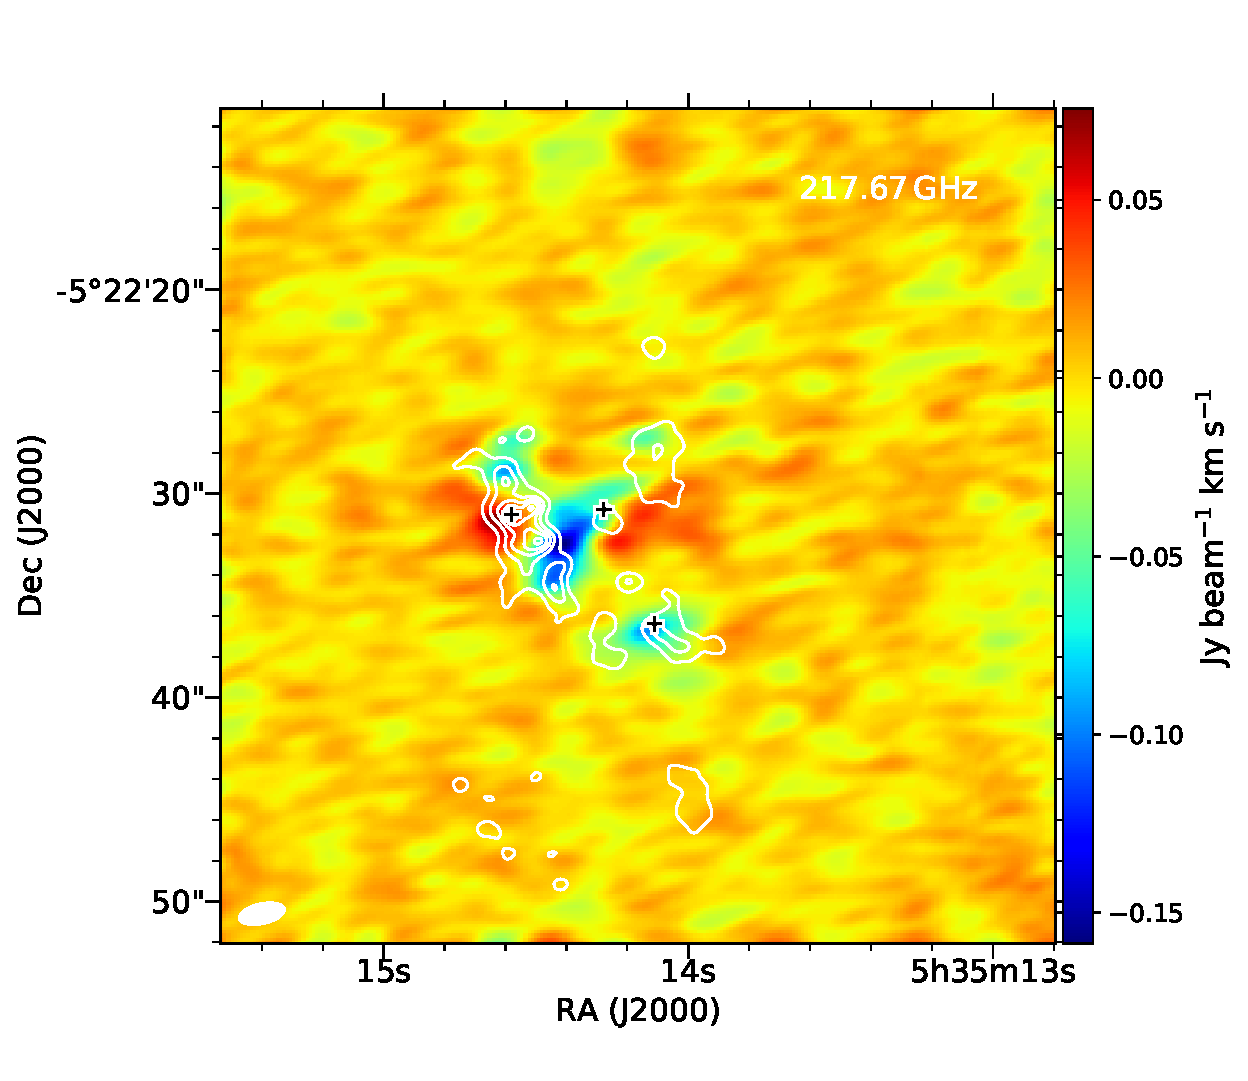
\includegraphics[width=0.98\textwidth]{OrionKL/mom0/217.67mom0_3-7.eps}
%\\(e) 左の図の説明
\end{center}
\end{minipage}
\begin{minipage}{0.48\textwidth}
\begin{center}
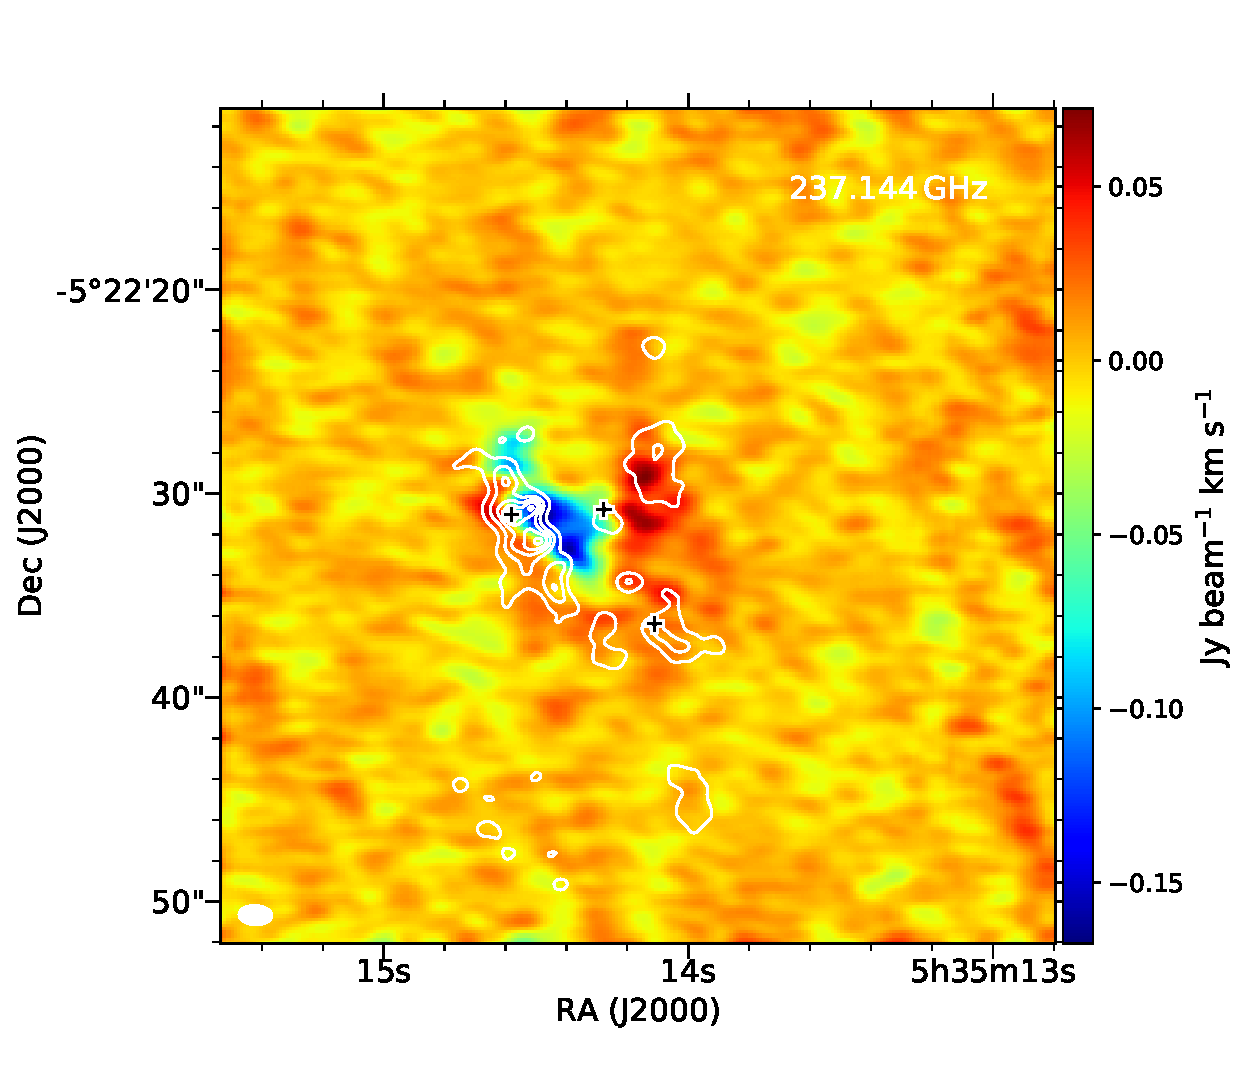
\includegraphics[width=0.98\textwidth]{OrionKL/mom0/237.144mom0_3-7.eps}
%\\(f) 右の図の説明
\end{center}
\end{minipage}
\end{center}
\end{minipage}
%%%% ここまで一組

\caption{(Continued)}
\end{center}
\end{figure}
%%%%%% ここまで

\newpage

\section{Channel maps}

\begin{figure}[htbp]
  \centering
  \includegraphics[width=0.98\textwidth]{OrionKL/chmap/222.846.eps}
  \caption{222.846GHz}
  \label{ap_ch_1}
\end{figure}

\begin{figure}[htbp]
  \centering
  \includegraphics[width=0.98\textwidth]{OrionKL/chmap/227.545.eps}
  \caption{227.545GHz}
  \label{ap_ch_2}
\end{figure}

\begin{figure}[htbp]
  \centering
  \includegraphics[width=0.98\textwidth]{OrionKL/chmap/231.844.eps}
  \caption{231.844GHz}
  \label{ap_ch_3}
\end{figure}

\begin{figure}[htbp]
  \centering
  \includegraphics[width=0.98\textwidth]{OrionKL/chmap/242.625.eps}
  \caption{242.625GHz}
  \label{ap_ch_4}
\end{figure}

\begin{figure}[htbp]
  \centering
  \includegraphics[width=0.98\textwidth]{OrionKL/chmap/231.524.eps}
  \caption{231.524GHz}
  \label{ap_ch_5}
\end{figure}

\begin{figure}[htbp]
  \centering
  \includegraphics[width=0.98\textwidth]{OrionKL/chmap/218.221.eps}
  \caption{218.221GHz}
  \label{ap_ch_6}
\end{figure}

\begin{figure}[htbp]
  \centering
  \includegraphics[width=0.98\textwidth]{OrionKL/chmap/219.151.eps}
  \caption{219.151GHz}
  \label{ap_ch_7}
\end{figure}

\begin{figure}[htbp]
  \centering
  \includegraphics[width=0.98\textwidth]{OrionKL/chmap/227.997.eps}
  \caption{227.997GHz}
  \label{ap_ch_8}
\end{figure}

\begin{figure}[htbp]
  \centering
  \includegraphics[width=0.98\textwidth]{OrionKL/chmap/231.061.eps}
  \caption{231.061GHz}
  \label{ap_ch_9}
\end{figure}

\begin{figure}[htbp]
  \centering
  \includegraphics[width=0.98\textwidth]{OrionKL/chmap/233.802.eps}
  \caption{233.802GHz}
  \label{ap_ch_11}
\end{figure}

\begin{figure}[htbp]
  \centering
  \includegraphics[width=0.98\textwidth]{OrionKL/chmap/231.576.eps}
  \caption{231.576GHz}
  \label{ap_ch_12}
\end{figure}

\begin{figure}[htbp]
  \centering
  \includegraphics[width=0.98\textwidth]{OrionKL/chmap/216.843.eps}
  \caption{216.843GHz}
  \label{ap_ch_13}
\end{figure}


\begin{figure}[htbp]
  \centering
  \includegraphics[width=0.98\textwidth]{OrionKL/chmap/251.128.eps}
  \caption{251.128GHz}
  \label{ap_ch_14}
\end{figure}

\begin{figure}[htbp]
  \centering
  \includegraphics[width=0.98\textwidth]{OrionKL/chmap/218.409.eps}
  \caption{218.409GHz}
  \label{ap_ch_15}
\end{figure}

\begin{figure}[htbp]
  \centering
  \includegraphics[width=0.98\textwidth]{OrionKL/chmap/217.67.eps}
  \caption{217.670GHz}
  \label{ap_ch_16}
\end{figure}

\begin{figure}[htbp]
  \centering
  \includegraphics[width=0.98\textwidth]{OrionKL/chmap/237.144.eps}
  \caption{237.144GHz}
  \label{ap_ch_17}
\end{figure}
%\thispagestyle{empty}\mbox{}\newpage

%%% acknowledgment %%%
\chapter*{Acknowledgments}
\addcontentsline{toc}{chapter}{Acknowledgments}

This work would have been never completed if anyone of greatest persons and colleagues mentioned below is missing.

I would like to express my gratitude my supervisor, Associate Professor Hideko Nomura, for her great
directions, fruitful discussions, and persistent encouragement.
I would like to do the same to Dr. Tomoya Hirota and Dr. Masatoshi Oh'ishi, who led me to the field of radio astronomy.
As for the data analysis of the ALMA telescope, Dr. Yoko Oya, Dr. Toshiki Saito, and Dr. Ryohei Kawabe gave me elaborate guidance.
I also received generous warm support and comments from Dr. Taiki Suzuki, Seongjoong Kim, and Wei Chen-en.

Finally, I am grateful to all of the colleagues of planetary groups at Tokyo Tech, and the seminar mates of ALMA interferometer seminar at National Astronomical Observatory of Japan (NAOJ) for scientific discussion and enjoyable life.


%\thispagestyle{empty}\mbox{}\newpage


%% 本編終了


%% referenceの表示

\addcontentsline{toc}{chapter}{References}

\bibliographystyle{apj}
\bibliography{references}%{references.bib}




\end{document}
